\documentclass[a4paper, 12pt, oneside]{book}
\usepackage{microtype} %used to manage hyphenations
\usepackage[utf8]{inputenc}% for the accents
\usepackage[T1]{fontenc}
\usepackage{mathptmx}
\usepackage{graphicx}
\usepackage{afterpage}
\usepackage{mathtools}
\usepackage{amsmath}
\usepackage{amsfonts}
\usepackage{xspace}
\usepackage{float} %to control the floating environments
\usepackage{appendix}
\usepackage[font={normal, it}, labelfont={bf, it}]{caption}
\usepackage[a4paper, inner=2.54cm, outer=2.54cm, top=2.54cm, bottom=2.54cm, bindingoffset=1cm]{geometry}
\frenchspacing
\renewcommand{\bibname}{References}
\setcounter{tocdepth}{3}

%temporary packages
\usepackage[english]{babel}
\usepackage{blindtext}
% \usepackage{titlesec}
%
% \titleclass{\chapter}{straight}
%using one half spacing between lines.
\usepackage[onehalfspacing]{setspace}

\usepackage{paralist}
\usepackage{hyperref}
\usepackage{cleveref}

\usepackage{array}
\usepackage{booktabs}


\newcommand{\head}[1]{\textbf{#1}}
\newcommand{\yhat}{\hat{y}}
\setlength{\abovetopsep}{1pt}
\DeclareUnicodeCharacter{2212}{-}

\begin{document}
\frontmatter
%the entire document will be divided into chapters only.
\chapter*{Abstract}
\blindtext
\addcontentsline{toc}{chapter}{Abstract}
\nopagebreak

\chapter*{Acknowledgment}
\blindtext
\addcontentsline{toc}{chapter}{Acknowledgment}

\tableofcontents
\addcontentsline{toc}{chapter}{\contentsname}
\listoftables
\addcontentsline{toc}{chapter}{\listtablename}
\listoffigures
\addcontentsline{toc}{chapter}{\listfigurename}
\addtocontents{toc}{\bigskip}

\chapter{List of Abbreviations}

\begin{description}

  \item[CNN] Convolutional neural networks
  \item[ANN] Artifitial neural networks

\end{description}

\mainmatter

\chapter*{Introduction}

The world nowadays is moving towards automation at an unprecedented rate. Almost every month, a new break-through is made in the path towards creating smart computer systems with the ability to learn and make decisions of their own. This progress does not only manifest itself in theoretical work and research papers, but also in real world applications such as the latest voice recognition software found in Amazons' Alexa, or the computer vision systems used by Teslas' autonomous cars. Most experts and speculators predict that soon enough, all of the aspects of ordinary life will be dependent upon the use of these artificially intelligent machines. Some are optimistic and consider this as a practical solution for a wide range of problems in various fields such as medicine, transportation, telecomunication, and even politics and economics. Others express fears that this technology may produce more problems that it would solve. In either case, the best way for academics to approach this is to explore this technology and develop a better understanding of the theory and methodology surrounding it.

This work is an attempt to bring a contribution to the field, and specifically the topic of deep convolutional neural networks, by developing a real world application to identify Algerian license plate numbers using image input of the cars. The techniques used are relatively outdated considering the high rate of innovation in deep learning. The two main research papers that this work is based upon came out in 2016 and 2018. The first one is a CNN model called Faster-RCNN and the other one is called YOLO, both these works showed practical state of the art results in the tasks of object detection and classification during the time they were released. This project also includes the creation of a lebeled data set of Algerian license plates, which is the first one ever of this kind. This data set will allow for other students or researchers to conduct similar works and will be used as a benchmark to track advancements in Algerian License plate detection.

\addcontentsline{toc}{chapter}{Introduction}
\chapter{Feed-Forward neural networks}
To understand the technique used in this report, it is necessary to understand basic neural networks functioning.
Given a scenario with a training set of labeled data $(\textbf{x}, \textbf{y})$, where $\textbf{x}$ denotes the training example
composed of multiple features, say $\textbf{x} = \{x_{1}, x_{2}, \ldots, x_{n}\}$, and \textbf{y} the corresponding label.
Let's introduce the idea of `perceptron'. \\
Perceptrons are the building blocks of neural networks, and the best way to get stated is with an example.
Assume at the university's admission office the students are evaluated with two pieces of information, the results of a test and their grades in school. Let's take a look at some sample students, see \cref{fig:perceptron}.

\begin{figure}[ht]
  \centering
  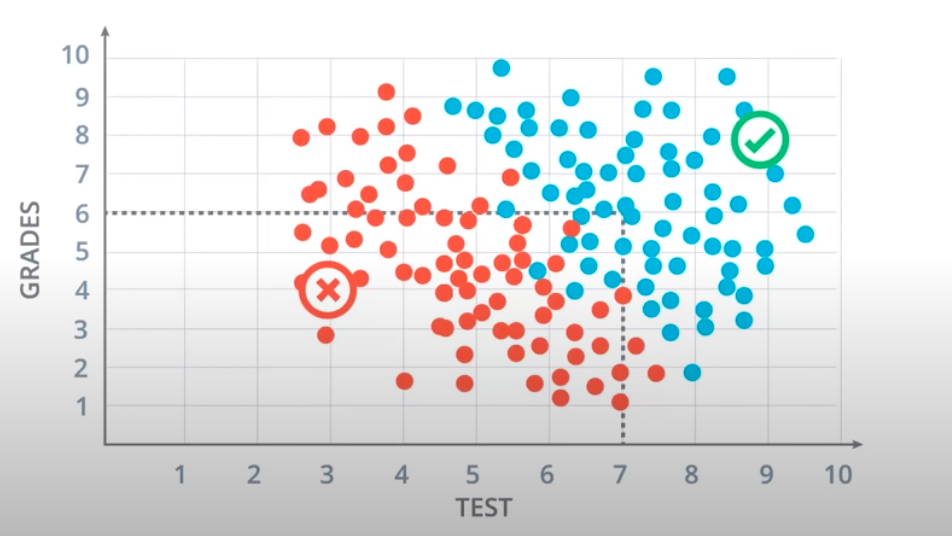
\includegraphics[width=0.7\textwidth]{figs/fig1.png}
  \caption{test vs grades }\label{fig:perceptron}
\end{figure}

The data on the figure can be nicely separated with a line, where most students above the line get accepted and most students under the line get rejected, see \cref{fig:line}. Therefore this line is going to be our model. \\
The model makes a couple of mistakes since there are a few blue points that are under the line and few over the line, but they are considered as noise and add no new information to our model. Now, the natural question that arises: how do we find the line ?

\begin{figure}[htbp]
  \centering
  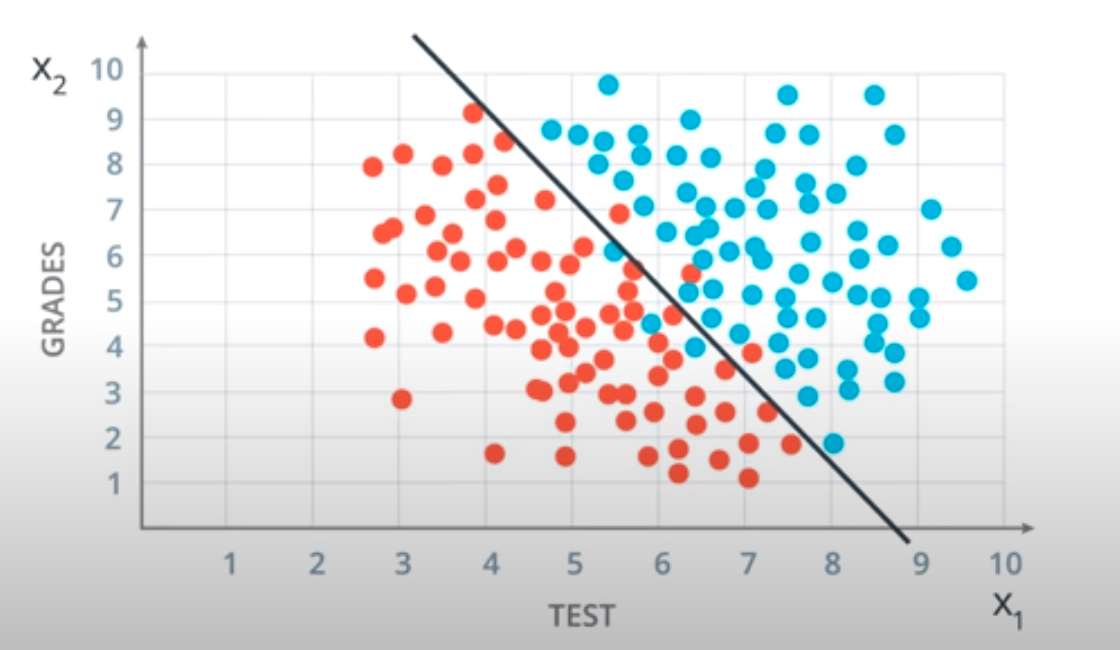
\includegraphics[width=0.7\textwidth]{figs/fig2.png}
  \caption{seperating line}\label{fig:line}
\end{figure}

We start by labeling the axis $\textbf{x} = \{x_{1}, x_{2}\}$.
The boundary line separating the students has a linear equation
specifically: $2x_{1} + x_{2} - 18 = 0$.
Plotting the grades in the equation gives rise to a score, if the score is positive --the student
gets plotted in above the line--, the student gets accepted with otherwise not. This is called a prediction.\\

In a more general case, our boundary will be an equation of the following form:

$$w_{1}x_{1} + w_{2}x_{2} + b = 0.$$

Abbreviating this equation into vector notation:

\begin{equation}
  \label{linear}
  \textbf{w}\cdot\textbf{x} + b = 0
\end{equation}

Where $\textbf{w} = \{w_{1}, w_{2}\}$. We refer to $\textbf{x}$ as the input, $\textbf{w}$ as the weights and $b$ as the bias. Here $\textbf{y} = \{0, 1\}$ is the label, where 0 indicates the student being rejected whereas 1 indicates the student being accepted. Finally, our prediction is going to be called \mbox{\boldmath{$\hat{y}$}} and it will be what the algorithm predicts that the label will be, namely:

\begin{equation}
  \label{y_hat}
  \hat{y} =
  \begin{dcases*}
    \text{1,}  &$w\cdot x + b \geq 0$ \\
    \text{0,}  &$w\cdot x + b < 0$
  \end{dcases*}
\end{equation}

and the goal of the algorithm is to have \mbox{\boldmath{$\hat{y}$}} resembling \mbox{\boldmath{$y$}} as closely as possible. Reorganizing the equations in a graph and generalizing, gives rise to \cref{fig:neuron}. Here the bias is consider as a dummy input with value 1 to the Perceptron with weight b.

% \afterpage{\cleardoublepage}
\begin{figure}[H]
  \centering
  \includegraphics[width=0.7\textwidth]{figs/perceptron.png}
  \caption{perceptron's graph representation}\label{fig:neuron}
\end{figure}

% \section{activation functions}
%
% Giving a training set, the classification of the input vector is based upon $\textbf{w}$, therefore the goal of the algorithm is to determine those
% weights through an iterative process. The probelm given here is that the algorithm can only learn linear functions since the output of the perceptron
% is a simple linear combination of the input. In real world situation, the data is much more complex and highly non-linear, therefore to remedy this
% problem we shall introduce a non-linearty in our algorithm, called \textbf{activation function} in deep learning literature. Namely the sigmoid
% function.
%
% $$
% \sigma(x) = \frac{1}{1 + e^{-x}}
% $$
%
% One important property of an activation function is differentiability, because as we are going to explore in section, gradient descent will be used as optimizer to determine the networks' weights, in contrast to the perceptron which uses a discrete activation. That sigmoid function can be seen as continuous version of the perceptron's discrete activation function. Indeed:
%
%
%
%
% Instead of returning 0 or 1, the sigmoid function returns the probability of an event occuring, thus in our example the sigmoid function would output
% the probability of a student getting accepted or rejected, which can be expressed as the the conditional probability $p(y=1 | x) = \sigma(w\cdot x +
% b)$. There several other activation functions that can be used depending on the problem at hand. For example if a neural network is used to predict
% continuous non-bounded function that takes values in the interval $]-\infty, +\infty[$, then a more clever choice is the linear activation
% funciton, which is defined as: $f(x) = x$.


\section{Cost function}\label{cost}

In order to estimate the accuracy of the algorithm, or otherwise stated determine how well a certain prediction given by the algorithm is, we may establish a cost function, which measures the error the algorithm makes on some prediction (cost function is often referred to as error function). There are more that one choice for such a function. \Cref{equ:mse} can be used, it is called ``The Mean Squared Error''.

\begin{equation}
  \label{equ:mse}
  L(w, b) = \frac{1}{2} \sum_{i = 1}^{n} ||y - \hat{y}||^2.
\end{equation}

This function, becomes large when our network approximates $y$ badly, and small when the approximation is accurate. Additionally notice that if we set $L_x = \frac{1}{2} (y - \hat{y})^2$ we have that:
\begin{equation}
  \label{equ:additivity}
  L(w,b) = \sum_{i = 1}^{n} L_{x_{i}}.
\end{equation}
This property will be important in the algorithm described in Section 2.2.3.

Another way of defining a cost function is using the ``The Maximum Likelihood Estimation'' technique, since the sigmoid function deals with probabilities. We take the joint probability of the entire training set, assuming the training examples being independent events:

\begin{equation}
  \label{equ:likelihood}
  L(w, b) = p(y^{(1)}, y^{(2)}, \ldots, y^{(n)} | x^{(1)}, \ldots, x^{(n)}) = \prod_{i=1}^{n} p(y^{(i)}|x^{(i)})
\end{equation}

where $x^{(i)}$, $y^{(i)}$ represent the $i^{th}$ training example and label respectively. Thus by maximizing the joint probability, or respectively minimizing the $-\log$ of the likelihood, we can get an estimate of the parameters $w \ and \ b $. Now, in our worked example, the neural network can be treated as a random variable having a Bernoulli distribution, therefore \cref{equ:likelihood} can be rewritten as follows:

\begin{equation}
  \label{equ:b_likelihood}
  L(w, b) = - \sum_{i = 1}^{n} y_i \log(\hat{y}) + (1 - y) \log(1 - \hat{y}).
\end{equation}

\Cref{equ:b_likelihood} is usually the cost function used for Bernoulli distributed labeled data. It is often referred to as \textbf{binary cross-entropy} or BCE for short.

For multi-class classification (predicting multiple classes, say $k$ classes), a similar idea can used considering a multinoulli distribution on the data set where $p(y | \textbf{x}) = \prod_{i = 1}^{k} p_i^{[y=i]}$, where $[y = i]$ evaluates to 1 if $x = i$, 0 otherwise. This leads to following cost function using MLE

\begin{equation}
  \label{equ:m_likelihood}
  L(w, b) = - \sum_{j = 1}^k \sum_{i = 1}^{n} y_{i, j} \log(\hat{y}_{i, j}).
\end{equation}

\section{Gradient descent}
In order to minimize the cost function we rely on optimization algorithms from numerical methods as it is unpractical to solve manually. The technique used in deep learning is the gradient descent. \\
The gradient of a differentiable function $f: \mathbb{R}^n \longrightarrow \mathbb{R}$ at a point $x = (x_1, \ldots, x_n) \in \mathbb{R}^n$ is a vector in $\mathbb{R}^n$ of the form

\begin{equation}
  \label{equ:gradient}
  \nabla f(x) = (\frac{\partial f}{\partial x_1} (x), \ldots, \frac{\partial f}{\partial x_n} (x))
\end{equation}

It is a well known result that, given a point $x \in \mathbb{R}^n$, the gradient at that point the direction of steepest ascent. Given that $f$ is differentiable at $x$, the vector $-\nabla f(x)$ indicates the direction of steepest descent of the function $f$ at the point $x$.
In order to obtain the minimum value of the function, the gradient descent strategy tells us to start at a given $x_0 \in \mathbb{R}^n$, calculate the value of $\nabla f(x_0)$, and then proceed to calculate a new point $x_1 = x_0 − \alpha \nabla f(x_0)$, where $\alpha > 0$ is called the \textbf{learning rate}. We then repeat this process, creating a sequence $\{ x_i \}$ defined by our initial choice of $x_0$, the learning rate $\alpha$, and the rule: $x_{i + 1} = x_{i} − \alpha \nabla f(x_0)$  . This sequence continues until we approach a region close to our desired minimum.
The method of gradient descent when taken continuously over infinitesimally small increments (that is, taking the limit $\alpha \rightarrow 0$) usually converges to a local minimum. However, depending on the location of the initial $x_0$, the local minimum achieved may not be the global minimum of the function. Furthermore, since when carrying out calculations on an unknown function we must take discrete steps (which vary in length depending on the learning rate), we are not even guaranteed a local minimum but rather may oscillate close to one, or even ’jump’ past it altogether if the learning rate is too big. Still, even with these possible complications, gradient descent is a surprisingly successful method for many real life applications and is the most standard method of training for feed-forward neural networks and many other machine learning algorithms.
Given that our cost function indicates how poorly our neural network approximates a given function, by calculating the gradient of the cost function with respect to the weights and biases of the network and adjusting these parameters in the direction opposite to the gradient, we will decrease our error and therefore lead us closer to an adequate network (in most cases) see .

\subsection{Gradient calculation}\label{sec:cal_gradient}

Before applying the gradient descent technique, we can clearly see that the an output of 0 or 1 is problematic since the derivatives would be 0. Therefore the gradient descent technique will not work. To remedy this, following the MLE, a Bernoulli distribution has been defined on $y$, therefore the neural net needs to predict $\yhat = p(y = 1 | x) = \sigma (x)$. For this number to be a valid probability, it must lie in the interval $[0, 1]$. \\
A good approach would ensure the existence of a strong gradient whenever the model has the wrong answer. And for consistency with the perceptron's decision rule (\cref{y_hat}), a very positive linear combination of the input $x$ has to have a probability close to 1 and vise versa (see \cref{fig:step_sigmoid}), otherwise

\begin{equation}
  \label{equ:limits}
  \lim_{x \rightarrow +\infty} \sigma(x) = 1, \qquad \lim_{x \rightarrow -\infty} \sigma(x) = 0.
\end{equation}

This approach is based on the sigmoid function:
 $$
 \sigma(x) = \frac{1}{1 + e^{-x}}
 $$

This function is suitable for the problem at hand, namely binary classification. However, depending on the output $\yhat$ other functions might be used. For example if a neural network is used to predict continuous non-bounded function that takes values in the interval $]-\infty, +\infty[$, then a more clever choice is the linear activation function, which is defined as: $f(x) = x$. Another example is the multi-class classification, where a multinoulli distribution is defined over the training data. The function used is the softmax defined as

$$
softmax(x_i) = \frac{e^{x_i}}{\sum_j e^{x_j}}
$$

Where $x_i$ represents a training example from class $i$. Here the output consists of $j$ outputs rather that a single one. See \cref{fig:ann} to illustrate the output layer.

\begin{figure}[!htpb]
  \centering
  \includegraphics[width=\textwidth]{figs/step_sigmoid.png}
  \caption[sigmoid vs step function]{sigmoid vs step function. The two plots clearly show cast the continuity of the sigmoid.}\label{fig:step_sigmoid}
\end{figure}

Now, let us apply the gradient descent technique to our network. Our goal is to calculate the gradient of $L$ at a point $x = (x_1, \ldots, x_n)$ given by the partial derivatives, see \cref{equ:gradient}. In addition, the property \cref{equ:additivity} now become important. In fact, we are only going to calculate the value of $\nabla L_x$ for a given labeled data point and then add the values of the gradient together, see below.

\begin{equation}
  \nabla L(w, b) = \nabla (\sum_{i = 1}^{n} L_x) = \sum_{i = 1}^{n} \nabla L_{x_i}.
\end{equation}

The error produced by each point is simply: $ L_x = -y \log (\hat{y}) - (1 - y) \log (1 - \hat{y})$. In order to calculate the derivative of this error with respect to the weights, we'll first calculate $ \frac{\partial}{\partial w_j} \hat{y}$, where $ \hat{y} = \sigma (w \cdot x + b)$.

\begin{align*}
  \frac{\partial}{\partial w_j} \hat{y} &= \frac{\partial}{\partial w_j} \sigma (w \cdot x + b) \\
     &= \sigma (w \cdot x + b) (1 - \sigma (w \cdot x + b)) \cdot \frac{\partial}{\partial w_j} (w \cdot x + b) \\
     &= \hat{y} (1 - \hat{y}) \cdot \frac{\partial}{\partial w_j} (w \cdot x + b) \\
     &= \hat{y} (1 - \hat{y}) \cdot \frac{\partial}{\partial w_j} (w_1 x_1 + \ldots + w_j x_j + \ldots w_n x_n + b) \\
     &= \hat{y} (1 - \hat{y}) \cdot x_j.
\end{align*}

Now we can go ahead and calculate the derivative of the error $L$ at a point $x$, with respect to the weight $w_j$.

\begin{align*}
  \frac{\partial}{\partial w_j} L_x &= \frac{\partial}{\partial w_j} [-y \log (\hat{y}) - (1 - y) \log (1 - \hat{y})] \\
     &= -y \frac{\partial}{\partial w_j} \log (\yhat) - (1 - y) \frac{\partial}{\partial w_j} (1 - \yhat) \\
     &= -y \frac{1}{\yhat} \cdot \frac{\partial}{\partial w_j} \yhat - (1 - y) \frac{1}{1 - \yhat} \cdot \frac{\partial}{\partial w_j} (1 - \yhat) \\
     &= -y (1 - \yhat) \cdot x_j + (1 - y)\yhat \cdot x_j \\
     &= -(y - \yhat) x_j
\end{align*}

A similar calculation will show that

$$
\frac{\partial}{\partial b} L_x = -(y - \yhat)
$$

Therefore, since the gradient descent step simply consists in subtracting a multiple of the gradient of the error function at every point, then this updates the weights in the following way:

\begin{align}
  w^{\prime}_i &= w_i + \alpha (y - \yhat)x_i \\
  b^{\prime} &= b + \alpha (y - \yhat)
\end{align}

\section{Neural network architecture}
In our work example, the target function was a simple linear function. However, in real world situations the input data is much more complex and often cannot be separated with a line. That is where neural nets shine. Neural networks also referred to as \textbf{feedforward} neural nets or \textbf{multilayer perceptron} (MLPs) are as the name indicates are stacks of perceptrons, where each \textbf{unit} receives the input $x$, calculates the inner product with a set of weights and apply a non-linearity to the result, then these results are fed to a next layer of units that does the same calculations and so on. The overall length of the chain gives the \textbf{depth} of the model. The final layer of such a network is called the \textbf{the output layer}, whereas the intermediate layer are referred to as \textbf{hidden layers}. The goal of the feed-forward network is to approximate some function $f^*$. The training example specify directly what the output layer must do at each point $x$; it must produce a value that is close to $y$. Therefore, the function computed after the linear combination is important. This function and the functions used in the hidden layers are referred to as \textbf{activation functions}. For example for a classifier, the function maps an input $x$ to a category $y$, a natural choice of activation is the sigmoid; whereas in a regression problem, where the output is continuous non-bounded that takes values in the interval $]-\infty, +\infty[$, a more clever choice is the linear activation function, which is defined as: $f(x) = x$.
The figure below depicts the architecture described above.

\begin{figure}[!htpb]
  \centering
  \includegraphics[width=\textwidth]{figs/nn.png}
  \caption[A visual representation of a feed-forward network]{A visual representation of a feed-forward network which approximates some function $f : \mathbb{R}^n \longrightarrow \mathbb{R}^m$ by
    computing the function $f^*(x) = (f^*_1(x), \ldots, f^*_m(x))$. In this approach, the network is shown as a
    directed weighted graph. Here $x = (x_1, \ldots, x_n)$}\label{fig:ann}
\end{figure}

For notation, set $w^n_{a, b} \in \mathbb{R}$ as the weight between the $a^th$ unit in the $(n - 1)^th$ layer with $k$ units to the $b^th$ unit in the $n^th$ layer with $j$ units.

\begin{equation}
  w_n = \begin{pmatrix}
    w^n_{1, 1} & \ldots & w^n_{1, k} \\
    \vdots & \ddots & \vdots \\
    w^n_{j, 1} & \ldots & w^n_{j, k}
  \end{pmatrix}
\end{equation}

The bias can be added as a dummy unit with input $x_{n+1} = 1$, which is a constant $b \in \mathbb{R}^j$. In order to calculate the output $a_n$ of the $n^th$ layer, we use the formula

$$
a_n = \sigma (w_n \cdot a_{n - 1} + b_n).
$$

In the above equation, the activation function $\sigma$ is applied element-wise to each element of the resulting vector. As the computations are carried out along the network's layers, the final function $f$ calculated by a network of depth $N$ is

$$
f(x) = \sigma(w_N\sigma(\ldots\sigma (w_2 \sigma(w_1 \cdot x + b_1) + b_2)) + b_N)
$$

\section{Back-propagation}
In order to train a neural network, the same techniques are used as in \cref{sec:cal_gradient}. First we define a cost function (which is the same as in the perceptron algorithm \cref{equ:b_likelihood},but with a much more complex $\yhat$), we calculate the feed-forward pass (we calculate the output $\yhat$), and then calculate the the gradient of the cost function $L$ with respect to every single weight and bias in the network, we get the following gradient vector $\nabla L = (\ldots, \frac{\partial}{\partial w^l_{i, j}} L, \ldots)$. Then applying the gradient step look likes

\begin{align*}
  w^{\prime l}_{i, j} &= w^l_{i, j} - \alpha  \frac{\partial}{\partial w^l_{i, j}} L\\
  b^{\prime l}_j &= b_j - \alpha \frac{\partial}{\partial b^l_j} L
\end{align*}

The big challenge of applying gradient descent to neural networks is calculating these partial derivatives.  This is where back-propagation comes in. This algorithm first tells us how to calculate these values for the last layer of connections, and with these results then inductively goes "backwards" through the network, calculating the partial derivatives of each layer until it reaches the first layer of the network. Hence the name "back-propagation".

For the purpose of this section it is useful to consider the values of each layer before the activation function step. Consider

\begin{equation*}
  z^l_j = \sum_k w^l_{j, k} a^{l - 1}_k + b^l_j \qquad \text{so that} \qquad a^l_j = \sigma (z^l_j).
\end{equation*}

Additionally, we denote the following:

\begin{equation}
  \delta^l_j = \frac{\partial}{\partial z^l_j} L
\end{equation}

This value will be useful for propagating the algorithm backwards through the network and directly related to $\frac{\partial}{\partial w^l_{i, j}} L$ and $\frac{\partial}{\partial b^l_j} L$ by the chain rule. since

\begin{align}
  \frac{\partial L}{\partial w^l_{i, j}}  &= \frac{\partial L}{\partial z^l_j} \frac{\partial z^l_j}{\partial w^l_{i, j}} = \delta^l_j a^{l - 1}_i \\
  \frac{\partial L}{\partial b^l_j} &= \frac{\partial L}{\partial z^l_j} \frac{\partial z^l_j}{\partial b^l_j} = \delta^l_j.
\end{align}

The value $a^{l - 1}_j$ has already been calculated through the forward pass. The only remaining term to calculate is $\delta^l_j$ and we obtain our gradient. Our first step is calculating this value for the last layer of the network, that is, $\delta^N_j$ for a network with $N$ layers. Since $a^{N}_j = \sigma (z^N_j)$, again using the chain rule

\begin{equation}
  \delta^N_j = \frac{\partial L}{\partial a^N_j} \frac{\partial a^N_j}{\partial z^N_j} = \frac{\partial L}{\partial a^N_j} \sigma^{\prime}(z^N_j)
\end{equation}

which can be easily calculated by a computer if we know how to calculate $\sigma^{\prime}$ (which should be true for any practical activation function).

Now we will only need to "propagate" this backwards in the network in order to obtain $\delta^{N - 1}_j$. In order to do so, apply the chain rule once again

\begin{align*}
  \delta^{N - 1}_j &= \frac{\partial L}{\partial z^{N - 1}_j} \\
                   &= \sum_i^k \frac{\partial L}{\partial z^{N}_i} \frac{\partial z^N_i}{\partial z^{N - 1}_j} \\
                   &= \sum_i^k \delta^N_i \frac{\partial z^N_i}{\partial z^{N - 1}_j}.
\end{align*}

If we focus on the term $\frac{\partial z^N_i}{\partial z^{N - 1}_j}$, we find that
\begin{align*}
  \frac{\partial z^N_i}{\partial z^{N - 1}_j} & = \frac{\partial (\sum_k w^N_{i, k} a^{N - 1}_k + b^N_i)}{\partial z^{N - 1}_j} \\
                &= \frac{\partial (w^N_{i, j} \sigma (z^{N - 1}_j))}{\partial z^{N - 1}_j} \\
                &= w^N_{i, j} \sigma^{\prime} (z^{N - 1}_j)
\end{align*}

which, again, can be easily calculated by a computer given the network. Therefore

\begin{equation}
  \delta^{N - 1}_j = \sum_i^k \delta^L_i w^N_{i, j} \sigma^{\prime} (z^{N - 1}_j).
\end{equation}

This formula tells us how to calculate any $\delta^l_j$ in the network, assuming we know $\delta^{l+1}$. We finally developed a way to
calculate all the $\delta^l_j$ ’s, given that we know what the values of $\delta^{l + 1}_j$  are. Thus, by propagating this method backwards through the layers of the network we are able to find all our desired partial derivatives, and can therefore calculate the value of $\nabla L$ as a function of the weights and biases of the network and execute the method of gradient descent.

\section{Problems related to neural nets}

Neural networks are extremely powerful function approximators, but if care is not taken during the design of architecture since there are many parameter one can tune (depth, number of units in each layer, \ldots). Therefore, a complex design namely high number of units in each layer and a deep network can lead to \textbf{overfitting}. Over-fitting is the case where the overall cost is really small (The network is doing very well on the training set) but the generalization of the model to unseen data is poor and unreliable. There are many solutions proposed to break this effect such as dropout which consists of randomly zeroing the output of some units in each layer to force the algorithm to take different routes through the network and better generalize. \\
Another famous problem neural nets suffer from is \textbf{local minimum} problem, where the gradient descent optimizer might converge to a local minimum rather than the global one. But as deep learning is evolving, we now understand that at higher dimensions the chance of getting in such situation is very unlikely due to tremendous number of dimensions deep networks deals with. \\
Another issue in deep neural nets is the \textbf{vanishing gradients}. As we learned from backp-ropagation, each of the neural network's weights receive an update proportional to the partial derivative of the error function with respect to the current weight in each iteration of training. The problem is that in some cases, the gradient will be vanishingly small, effectively preventing the weight from changing its value. In the worst case, this may completely stop the neural network from further training. As one example of the problem cause, traditional activation functions such as the sigmoid function have gradients in the range (0, 1), and back-propagation computes gradients by the chain rule. This has the effect of multiplying $n$ of these small numbers to compute gradients of the "front" layers in an N-layer network, meaning that the gradient decreases exponentially with N while the front layers train very slowly.
To remedy this problem other activation functions might be used in the hidden layers. The behavior of the hidden layers is not directly
specified by the training data. The learning algorithm must decide how to use those layers to produce the desired output, but the training data do not say what each individual layer should do. Instead, the learning algorithm must decide how to use these layers to best implement an approximation of $f$. Therefore the choice of the activation function in those layers is irrelevant, which makes the use of other activation possible. Many functions have been proposed to escape the trap of vanishing gradients, namely the ReLU function is of popularity in deep learning. The ReLU stands for rectified linear unit defined as $ReLU(x) = \max (0, x)$.

\section{batch and stochastic gradient descent}

Batch gradient descent is just another name for the gradient descent discussed so far. It involves calculations over the full training set to take a single step as a result of which it is very slow on very large training data due to the size of the weight matrices that take up large memory portions. Thus it become very computationally expensive to do batch GD. One can take advantage of the property mentioned on \cref{cost}, \cref{equ:additivity}. Therefore, instead going through the entire data-set at each iteration we select a few elements from the
training set, commonly selected by randomly sampling from all the available labeled data, calculate the gradient, update the network's weights and repeat the process until the network arrives at satisfactory results. The gradients computations are faster as there is much fewer data to manipulate in a single time. This technique is referred to as \textbf{stochastic} gradient descent. One downside though of SGD is, once it reaches close to the minimum value then it does not settle down, instead bounces around which gives us a good value for model parameters but not optimal which can be solved by reducing the learning rate at each step which can reduce the bouncing and SGD might settle down at global minimum after some time.

\chapter[Convolution neural networks]{Neural network Variant: Convolutional Neural Networks}

Convolutional networks, also known as convolutional neural networks, or CNNs, are a specialized kind of neural network for processing data
that has a known grid-like topology. Examples include time-series data, which can be thought of as a 1-D grid taking samples at regular time intervals, and image data, which can be thought of as a 2-D grid of pixels. Convolutional networks have been tremendously
successful in practical applications. The name “convolutional neural network” indicates that the network employs a mathematical operation
called convolution. Convolution is a specialized kind of linear operation. Convolutional networks are simply neural networks that use
convolution in place of general matrix multiplication in at least one of their layers \cite{Ian16}.

\section{The convolution operation}

The convolution operation is well known in the engineering terminology, which, in its most general form, is an operation on two functions of a real-valued argument.
defined as:

\begin{equation}
  \label{convolution}
  s[n] = y[n] \ast x[n] = \sum_{k=-\infty}^{k=\infty} y[k] x[n - k]
\end{equation}

We are interested in the discrete convolution operation, since data on a computer is presented as discrete values rather than continuous
signals.
The \cref{convolution} presented above is for discrete time signals. \\

In convolution neural network terminology, the first argument to the convolution is often referred to as \textbf{the input}, and the second argument as \textbf{the kernel}.
The output is sometimes referred as the \textbf{feature map}. The input is usually a multidimensional array of data (RGB images), and the kernel is usually a multidimensional array of parameters that are adapted by the learning algorithm. These multidimensional arrays are referred as tensors. Finally, we often use convolution over more than one axis at a time.
For example if we use a two-dimensional image $I$ as our input, we probably also want to use a
two-dimensional kernel $K$:

\begin{equation}
  \label{2Dconvolution}
  S[m, n] = I[m, n] \ast K[m, n] = \sum_{i}\sum_{j} I[i, j] K[m - i, n - j].
\end{equation}

Convolution is commutative, meaning we can equivalently write:

\begin{equation}
  \label{2Dflipped}
  S[m, n] = K[m, n] \ast I[m, n] = \sum_{i}\sum_{j} I[m - i, n -j] K[i, j].
\end{equation}

While the commutative property is useful for writing proofs, it is not usually an important property of a neural
network implementation. Instead, many neural network libraries implement a
related function called the cross-correlation, which is the same as convolution
but without flipping the kernel:

\begin{equation}
  \label{cross-correlation}
  S[m, n] = I[m, n] \ast K[m, n] = \sum_{i}\sum_{j} I[m + i, n + j] K[i, j].
\end{equation}

Many machine learning libraries implement cross-correlation but call it convolution. See \cref{fig:conv-ex} for an example of convolution
applied to a 2d tensor (gray-scale image).


\begin{figure}[!htbp]
  \centering
  \includegraphics{figs/conv_ex.png}
  \caption{An example of 2-D convolution}\label{fig:conv-ex}
\end{figure}

\section{Convolution networks architecture}

Convolution leverages three important ideas that can help improve a machine learning system: sparse connectivity, parameter sharing and
equivariant representations.

Traditional neural network layers use matrix multiplication by a matrix of parameters with a separate parameter describing the interaction between each input unit and each output unit. This means that every output unit interacts with every input unit, see \cref{fig:fully_connected}.
Convolutional networks, however, typically have sparse interactions (also referred to as \textbf{sparse connectivity} or sparse weights).
This is accomplished by making the kernel smaller than the input.
For example, when processing an image, the input image might have thousands or millions of pixels, but we can detect small, meaningful features such as edges with kernels that occupy only tens or hundreds of pixels. This means that we need to store
fewer parameters, which both reduces the memory requirements of the model and improves its statistical efficiency.
It also means that computing the output requires fewer operations. These improvements in efficiency are usually quite large.
If there are $m$ inputs and $n$ outputs, then matrix multiplication requires $m \times n$
parameters, and the algorithms used in practice have $O(m \times n)$ runtime (per example).
If we limit the number of connections each output may have to $k$, then the sparsely connected approach requires
only $k \times n$ parameters and $O(k \times n)$ runtime. For many practical applications, it is possible to obtain good performance
on the machine learning task while keeping $k$ several orders of magnitude smaller
than $m$ \cite{Ian16}. For graphical demonstrations of sparse connectivity, see \cref{fig:s_conv_1} and \cref{fig:s_conv_2}.

\begin{figure}[!htbp]
  \centering
  \includegraphics{figs/fully_connected.png}
  \caption[Traditional neural network connections]{Traditional neural network connections. The last layer has been replace by a black box for simplicity}\label{fig:fully_connected}
\end{figure}

\begin{figure}[!htbp]
  \centering
  \includegraphics{figs/conv_1.png}
  \caption{Sparce connectivity}\label{fig:s_conv_1}
\end{figure}

Rearranging each vector as a matrix, the relationship between the nodes in each layer are more obvious, see \cref{fig:s_conv_2}.


\begin{figure}[!htbp]
  \centering
  \includegraphics{figs/conv_2.png}
  \caption{Sparce connectivity after rearrangement}\label{fig:s_conv_2}
\end{figure}

\textbf{Parameter sharing} refers to using the same parameter for more than one function in a model. In a traditional neural net, each
element of the weight matrix is used exactly once when computing the output of a layer. It is multiplied by one element of the input and
then never revisited. As a synonym for parameter sharing, one can say that a network has tied weights, because the value of the
weight applied to one input is tied to the value of a weight applied elsewhere \cref{fig:fully_connected}.
That is the reason, traditional nets are referred as to Fully connected (FC) networks or Dense networks.\\

In a convolutional neural net, each member of the kernel is used at every position
of the input (except perhaps some of the boundary pixels, depending on the
design decisions regarding the boundary). The parameter sharing used by the
convolution operation means that rather than learning a separate set of parameters
for every location, we learn only one set. In \cref{fig:s_conv_2}, each of the color coded image quarters are connected to a single color
coded node in the next layer. All of these connections have exactly the same shared weights, see \cref{fig:conv-ex}, the weights $w_{11}$
through $w_{33}$ do not change as the filter slides through the image. This does not affect the runtime of
forward propagation—it is still $O(k \times n)$—but it does further reduce the storage
requirements of the model to $k$ parameters. The particular form of parameter sharing causes the
layer to have a property called \textbf{equivariance to translation}. \\

To say a function is equivariant means that if the input changes, the output changes in the same way.
Specifically, a function $f(x)$ is equivariant to a function $g$ if $f(g(x)) = g(f(x))$. In
the case of convolution, if we let $g$ be any function that translates the input, that
is, shifts it, then the convolution function is equivariant to $g$. For example, let $I$
be a function giving image brightness at integer coordinates. Let $g$ be a function
mapping one image function to another image function, such that $I^{\prime} = g(I)$ is the
image function with $I^{\prime}(x, y) = I(x - 1, y)$. This shifts every pixel of $I$ one unit to
the right. If we apply this transformation to $I$, then apply convolution, the result
will be the same as if we applied convolution to $I$, then applied the transformation
$g$ to the output. With images, convolution creates a 2-D map of where certain features appear in the input. If we move the object in the
input, its representation will move the same amount in the output. This is useful for when we know that some function of a small number of
neighboring pixels is useful when applied to multiple input locations. For example, when processing
images, it is useful to detect edges in the first layer of a convolutional network.
The same edges appear more or less everywhere in the image, so it is practical to share parameters across the entire image. \\

Convolution is not naturally equivariant to some other transformations, such as changes in the scale or rotation of an image. Other
mechanisms are necessary for handling these kinds of transformations. To illustrate these principles in action, we shall use a hand picked
filter that used to detect edges in a image, see below.

$$
K = \begin{pmatrix}
0  & -1  &  0 \\
-1 &  4  & -1 \\
0  & -1  &  0
\end{pmatrix}
$$

These filters are called high pass filters. They enhance high frequency components in an image. Frequency in images just like in signals is the rate
of change of the intensity, which areas in neighboring pixels that rapidly changes for example from very dark to very light (in grayscale images).
See \cref{fig:filter} to see the effect of applying the above filter to a grayscale image.

\begin{figure}[H]
  \centering
  \includegraphics[width=0.8\textwidth]{figs/panda.png}
  \caption[2D convolution]{2D convolution. Where there is no change or little change of intensity in the original picture, the high pass filter
  block those areas out and turn the pixels black. But in the areas where a pixel is way brighter than its immediate neighbors, the high pass filter
  enhance the change and create a line. This has the effect of emphasizing edges. Edges are just areas in an image where the intensity changes very
  quickly. This images has been obtain by convolving the filter $K$ with the image in the left, as we can see the three principles discussed above
  apply to this filter. The values of $K$ didn't change while convolving (shared parameters). Space connectivity where
  the filter looks only to a small portion of the image at a time. And the equivariant translation, where we clearly see that no matter the position
  of the edge in the image the filter successful highlight it.}\label{fig:filter}
\end{figure}

\section{Convolutional layer}

The convolutional layer is produced by applying a series of many different image filters, also known as convolutional kernels, to an input image.

\begin{figure}[!htbp]
  \centering
  \includegraphics{figs/filters.png}
  \caption{Multiple filters for mutiple pattern detection}
\end{figure}

In the example shown, 4 different filters produce 4 differently filtered output images.
When we stack these images, we form a complete convolutional layer with a depth of 4. See \cref{fig:conv_layer}.

\begin{figure}[!htbp]
  \centering
  \includegraphics{figs/conv_layer.png}
  \caption{A complete convolutional layer with 4 filters}\label{fig:conv_layer}
\end{figure}

In case of colored images, computer interprets them as 3D-tensor $(Height \times width \times channels)$. Here channels are the RGB channels. When
performing convolution, the kernel $K$ is itself chosen to be three dimensional as well. A typical kernel $K$ would be $3 \times 3 \times 3$. The
resulting output feature map would be $(Height \times Width)$. In order to depict multiple patterns in the image, instead of having a single kernel,
multiple kernel are defined. Now each resulting output feature map can be considered as an image channel and stack them to get a 3 dimensional
array. The latter 3D array can be used as input to another convolutional layer to discover patterns within the patterns that we discovered in the
first convolutional layer. This operation can be repeated multiple times to discover various patterns within the input image.

In CNNs, inference works the same way as old plain neural network. Both convolutional and Dense layers have weights and biases and initial
randomly generated. Therefore, in the case of CNNs where the weights take the form of convolutional kernel or filters, those kernels are randomly
generated and so are the patterns that they're initially designed to detect. As with Fully connected networks, when we construct a CNN, we will
always specify a loss function. In the case of multiclass classification, this will be categorical cross-entropy loss(equ  from chapter 1). Then as
we train the model through back propagation, the filters are updated at each iteration to take on values that minimizes the loss function. In other
words, the CNN determines what kind of patterns it needs to detect base on the loss function.

\section{Stride and padding}
The behavior of a convolutional neural network can be controlled by specifying the number of filters and the size of each filter, these are referred
to as \textbf{hyper-parameters}. For instance, to increase the number of nodes in a convolutional layer, you could increase the number of filters.
To increase the size of the detected patterns, you could increase the size of the filters. But there are more hyper-parameters than we can tune.
One of these hyper-parameters is referred to as the stride of the convolution. The stride is just the amount by which the filter slides over the
image. In the previous example \cref{fig:conv-ex}, the stride was one. We move the convolution window horizontally and vertically  across the image
one pixel at a time \cite{ud188}. The width and height of the output of the convolution is given by \cref{conv_out_1}, if the input image is $n \times n$,
with a filter $f \times f$ :

\begin{equation}
  \label{conv_out_1}
  n - f + 1 \times n - f + 1
\end{equation}

If we introduce the stride parameter $s$, \cref{conv_out_1} can be rewritten as follow:

\begin{equation}
  \label{conv_out_2}
  \lfloor\frac{n - f}{s}\rfloor + 1\times \lfloor\frac{n - f}{s}\rfloor + 1
\end{equation}


One downside of the convolution operation is the shrinking input dimensions. Indeed, according to \cref{conv_out_1}, the input dimension shrinks
each time by few pixels which can be an undesirable effect in very deep networks, where the image can shrink to very small dimensions. Another
downside of the convolution is, the top left pixel (or corners of an image in general) is only involved in one pass of the filter, whereas if we
take a pixel in the middle, then many $2 \times 2$ regions will overlap that pixel. It as if the pixels at the corners are used much less in the
output, so information is thrown away near the edge of the image. Therefore to solve both of this problems, before applying the convolution we can
pad the image with additional boarders, for instance 1 pixel, see \cref{fig:padding}. Therefore the width and height of the output feature map is
calculated as:

\begin{equation}
  \label{conv_out_3}
  \lfloor\frac{n - f + 2p}{s}\rfloor + 1 \times \lfloor\frac{n - f + 2p}{s}\rfloor + 1
\end{equation}

Now with this additional boarder of zeros, the output feature maps' dimensions can be made equal to the input's dimension by setting the
appropriate padding value. And the corner pixels contribute more in the output feature map.

\begin{figure}[H]
  \centering
  \includegraphics{figs/padding.png}
  \caption{Padding example.}\label{fig:padding}
\end{figure}

\section{Pooling}

Pooling function is the next type of layer in convolutional neural networks. It replaces the output of the net at a certain location with
a summary statistic of the nearby outputs. For example, the max pooling operation reports the maximum output within a rectangular
neighborhood. Other popular pooling functions include average pooling of a rectangular neighborhood \cite{Ian16}.
see figure  on how to perform max pooling.

\begin{figure}[!htbp]
  \centering
  \includegraphics{figs/max_pooling.png}
  \caption[Maxpooling example]{Maxpooling example. As in the convolution operation, we slide a window across the image typically a $2 \times 2$ window. The value of the
  corresponding node in the max pooling layer is calculated by just taking the maximum of the pixels contained in the window. The pooling function
  is applied independently on every feature map in the input stack. The output is a stack with same number of feature maps with width and height
  reduced by a factor of two.}\label{fig:maxpooling}
\end{figure}

In all cases, pooling helps to make the representation approximately invariant to small translations of the input. Invariance to translation means
that if we translate the input by a small amount, the values of most of the pooled outputs do not change. Invariance to local translation can be a
useful property if we care more about whether some feature is present than exactly where it is.For example, when determining whether an image
contains a face, we need not know the location of the eyes with pixel-perfect accuracy, we just need to know that there is an eye on the left side
of the face and an eye on the right side of the face. Another improvement that pooling brings is the computational efficiency of the network. The
reason being is that pooling reports summary statistics for regions spaced with stride $s$ (typically 2 is used), therefore the next layer has
roughly $s$ times fewer inputs to process and reduces the memory requirements for storing parameters \cite{Ian16}. \\

Therefore, most CNNs are composed of only those two layers: Pooling and convolution. We begin with convolution layers which detects regional patterns
in an image using a series of filters. Typically, just like fully connected networks, an activation function is applied to the output feature maps.
RelU activation function is used as it has proven to be extremely efficient in object classification tasks. Then pooling layers follow the
convolutional layers to reduce the dimensionality of their input tensors. CNNs are designed with the goal of taking an input image and gradually
making it much deeper than it is tall or wide. As the network gets deeper, it is actually extracting more and more complex patters and features that
help identify the content and objects in an image. CNNs are usually referred to as \textbf{feature extractors}. Another issue that rises when
training CNNs, is the input image dimensions. Since training requires large datasets of thousands of images, it no surprise that these images
are of different sizes and shapes. Therefore CNNs requires a fixed sized input due to batch training. Indeed, instead of passing one image at a time
through the network, we usually pass batches of images which are just stacks of images. But in order to do that, all the images have to have the
same width and height. So, we have to pick an image size and resize all of our images to that same size before doing anything else.

\section{Case studies}

So why look at case studies? In the few last chapters, we learned about the basic building blocks such as convolutional layers, pooling layers and fully connected layers of conv nets. It turns out a lot of the past few years of computer vision research has been on how to put together these basic building blocks to form effective convolutional neural networks. One of the best ways to get intuition on how to build conv nets is to read or to see other examples of effective conv nets, and it turns out that a net neural network architecture that works well on one computer vision task often works well on other tasks as well.

\subsection{VGG-16}

VGG16 is a convolutional neural network model proposed by K. Simonyan and A. Zisserman from the University of Oxford in the paper “Very Deep Convolutional Networks for Large-Scale Image Recognition”. The model achieves 92.7\% top-5 test accuracy in ImageNet, which is a dataset of over 14 million images belonging to 1000 classes. It was one of the famous model submitted to ILSVRC-2014. It makes the improvement over AlexNet by replacing large kernel-sized filters (11 and 5 in the first and second convolutional layer, respectively) with multiple $3 \times 3$ kernel-sized filters one after another. VGG16 was trained for weeks and was using NVIDIA Titan Black GPU’s. see \cref{fig:vgg16}.

\begin{figure}[!htpb]
	\centering
	\includegraphics[width=\textwidth]{figs/vgg16.png}
	\caption{vgg 16}\label{fig:vgg16}
\end{figure}

The ConvNet configurations are outlined in \cref{fig:vgg16_2}. The nets are referred to their names (A-E). All configurations follow the generic design present in architecture and differ only in the depth: from 11 weight layers in the network A (8 conv. and 3 FC layers) to 19 weight layers in the network E (16 conv. and 3 FC layers). The width of conv. layers (the number of channels) is rather small, starting from 64 in the first layer and then increasing by a factor of 2 after each max-pooling layer, until it reaches 512. see \cref{fig:vgg16_2}.

\begin{figure}[!htpb]
	\centering
	\includegraphics[width=0.8\textwidth]{figs/vgg16_2.png}
	\caption{vgg 16 config}\label{fig:vgg16_2}
\end{figure}

\subsection{Res-Net}

ResNet, short for Residual Networks is a classic neural network used as a backbone for many computer vision tasks. This model was the winner of ImageNet challenge in 2015. The fundamental breakthrough with ResNet was it allowed us to train extremely deep neural networks with 150+layers successfully. Prior to ResNet training very deep neural networks was difficult due to the problem of vanishing gradients.

AlexNet, the winner of ImageNet 2012 and the model that apparently kick started the focus on deep learning had only 8 convolutional layers, the VGG network had 19 and Inception or GoogleNet had 22 layers and ResNet 152 had 152 layers.

However, increasing network depth does not work by simply stacking layers together. Deep networks are hard to train because of the notorious vanishing gradient problem — as the gradient is back-propagated to earlier layers, repeated multiplication may make the gradient extremely small. As a result, as the network goes deeper, its performance gets saturated or even starts degrading rapidly. For this reason the creators of Res-Net introduced the idea of "Skip Connections"

\subsubsection{Skip Connection}

ResNet first introduced the concept of skip connection. \cref{fig:resnet1}. below illustrates skip connection. The figure on the left is stacking convolution layers together one after the other. On the right we still stack convolution layers as before but we now also add the original input to the output of the convolution block. This is called skip connection. We must note that the addition operation occures before the output goes through the ReLu function.
The main two reasons why skip connections work are :

\begin{itemize}
  \item They mitigate the problem of vanishing gradient by allowing this alternate shortcut path for gradient to flow through
  \item They allow the model to learn an identity function which ensures that the higher layer will perform at least as good as the lower layer, and not worse
\end{itemize}

\begin{figure}[!htpb]
	\centering
	\includegraphics[width=0.8\textwidth]{figs/resnet1.png}
	\caption{resnet1}\label{fig:resnet1}
\end{figure}

\subsection{Inception}

The Inception network was an important milestone in the development of CNN classifiers. Prior to its inception (pun intended), most popular CNNs just stacked convolution layers deeper and deeper, hoping to get better performance.The Inception network on the other hand, was complex (heavily engineered). It used a lot of tricks to push performance; both in terms of speed and accuracy. Its constant evolution lead to the creation of several versions of the network. The popular versions are : Inception v1, Inception v2, Inception v3, and Inception Res-Net. Each version is an iterative improvement over the previous one. Understanding the upgrades can help us to build custom classifiers that are optimized both in speed and accuracy.

\subsubsection{Inception V1}
The Problem addressed by the developers of this model is the extreme large variation in the size of the salient parts in the image. For instance, An image of a dog can have any of the forms shown in \cref{fig:inception1}. The area occupied by the dog is different in each image. This significant variation in the location of the relevant features of the object we wish to detect and classify requires choosing the right kernel size for the convolution operation, which becomes a complicated task. A larger kernel is preferred for information that is distributed more globally, and a smaller kernel is preferred for information that is distributed more locally. And considering the fact that very deep networks are prone to overfitting in addition to the difficulty they pose in performing back-propagation across the layers it goes without saying that naively stacking large convolution operations is computationally expensive and will not improve network performance on new data.

As a solution, the authors of the original paper suggested the use of multiple filters of different sizes in one layer. Rendering The network "wider" rather than “deeper”.

\Cref{fig:inception2} explains the core idea of this model. It performs convolution on an input, with 3 different sizes of filters $(1 \times 1, 3 \times 3, 5 \times 5)$. Additionally, max pooling is also performed. The outputs are concatenated and sent to the next inception layer.

As stated before, deep neural networks are computationally expensive. To make it cheaper, the authors limit the number of input channels by adding an extra $1 \times 1$ convolution before the $3 \times 3$ and $5 \times 5$ convolutions. Though adding an extra operation may seem counterintuitive, $1 \times 1$ convolutions are far less expensive than $5 \times 5$ convolutions, and the reduced number of input channels also help (similar to the method used in mobilenet). Do note that however, the 1x1 convolution is introduced after the max pooling layer, rather than before. See \cref{fig:inception3}


\begin{figure}[ht]
	\centering
	\includegraphics[width=0.9\textwidth]{figs/inception1.png}
	\caption{inception1}\label{fig:inception1}
\end{figure}

\begin{figure}[ht]
	\centering
	\includegraphics[width=0.9\textwidth]{figs/inception2.png}
	\caption{inception2}\label{fig:inception2}
\end{figure}

Using the dimension reduced inception module, a neural network architecture was built. This was popularly known as GoogLeNet (Inception v1). The architecture is shown in \cref{fig:inception4}.

\begin{figure}[ht]
	\centering
	\includegraphics[width=0.9\textwidth]{figs/inception3.png}
	\caption{inception3}\label{fig:inception3}
\end{figure}

\begin{figure}[ht]
	\centering
	\includegraphics[width=\textwidth]{figs/inception4.png}
	\caption{inception4}\label{fig:inception4}
\end{figure}

GoogLeNet has 9 such inception modules stacked linearly. It is 22 layers deep (27, including the pooling layers). It uses global average pooling at the end of the last inception module.

Needless to say, it is a pretty deep classifier. As with any very deep network, it is subject to the vanishing gradient problem.

To prevent the middle part of the network from “dying out”, the authors introduced two auxiliary classifiers (The purple boxes in \cref{fig:inception4}). They essentially applied softmax to the outputs of two of the inception modules, and computed an auxiliary loss over the same labels. The total loss function is a weighted sum of the auxiliary loss and the real loss. Weight value used in the paper was 0.3 for each auxiliary loss. Needless to say, auxiliary loss is purely used for training purposes, and is ignored during inference.
$$
total\ loss = real\ loss + 0.3\  aux\ loss_1 + 0.3\  aux\ loss_2
$$

\subsection{Mobilenet}
MobileNet is a CNN architecture model for used for object detection and image Classification, generally used in mobile applications.There exists a variety of models designed for the same purpose as well but the reason why MobileNet stand out is that it requires much less computation power to run or apply transfer learning to.This characteristic is what makes it optimal to run on embedded systems in general , computer systems without GPU or low computational efficiency, as well as Mobile devices which don't have the necessairy hardware to run more costly models. Needless to say, the use of Mobilenet  comes with a significant compromise in the accuracy of the results. It is also best suited for web browsers as browsers have limitation over computation,graphic processing and storage. Mobilenet architecture is distinguished by an essenstial features know as "Depthwise Separable Convolution".

\subsubsection{Depthwise Separable Convolution}
Before we get into the definition of "Depthwise Separable Convolution" we need to go over some aspects of the convolution operation. Let's consider an input matrix of shape $D_{f} \times D{f} \times M $ as shown in \cref{fig:dsc input}. If our input was an RGB image then M would be equal to 3. If we apply a convolution using a filter of shape $D_{k} \times D{k} \times M $ we would obtain an output of size $D_{G} \times D{G} \times 1 $ if we apply the same convolution using N filters of the same shape and concatenate the results we would obtain an output shape of $D_{G} \times D{G} \times N $, see \cref{fig:dsc conv1}.

\begin{figure}[ht]
	\centering
	\includegraphics[width=0.7\textwidth]{figs/dsc input.png}
	\caption{Convolution input }\label{fig:dsc input}
\end{figure}

\begin{figure}[ht]
	\centering
	\includegraphics[width=0.9\textwidth]{figs/dsc conv1.png}
	\caption{Convolution operation }\label{fig:dsc conv1}
\end{figure}

Since the multiplication operation is more expensive relative to the addition, let's consider the cost of the convolution operation with regards to the number of multiplications. For one convolution step for one kernal the number of multiplications is $D_{k} \times D_{k} \times M $, for and entire convolution step for one filter the number of multiplications is $D_{G} \times D_{G} \times D_{k} \times D_{k} \times M $ therefore when we account for N filters the number of multiplication for a convolutional layer is $D_{G}^{2} \times D_{k}^{2} \times M $
With this in mind, we can introduce the concepts of "Depthwise Convolution" and "Pointwise convolution", which when put together yeild a " Deapthwise Separable Convolution ". Unlike simple convolution, Deapthwise Convolution applies convolution to single input channel at a time, using M filters of shape  $D_{k} \times D_{k} \times 1 $ see \cref{fig:dsc conv2}. Pointwise convolution applies N filters of shape $1 \times 1 \times M $ to the output of the Deapthwise convolution and by concatenating the results we obtain the same output shape as simple convolution, see \cref{fig:dsc conv3}

\begin{figure}[ht]
	\centering
	\includegraphics[width=0.9\textwidth]{figs/dsc conv2.png}
	\caption{Deapthwise Convolution }\label{fig:dsc conv2}
\end{figure}

\begin{figure}[ht]
	\centering
	\includegraphics[width=0.9\textwidth]{figs/dsc conv3.png}
	\caption{Pointwise Convolution }\label{fig:dsc conv3}
\end{figure}

computing the number of multiplications for the entire process gives  $M \times D_{G}^{2} \times (D_{k}^{2}+N) $ Which is less than the cost of simple convolution. But to get a an understanding of how much computational power is reduced we should compute the ratio

$$
\frac{number\ of\ multiplications\ for\ DSC}{number\ of\ multiplications\ for\ simple\ conv}
$$

Which is found to be

$$
\frac{1}{N} + \frac{1}{D_{k}^2}
$$

By taking an example of $D_{k} = 3$ and $N = 1024$ we get a ratio of approximately $\frac{1}{9}$ which signifies a substantial decrease in computational requirements.

\subsubsection{Mobilenet model}

The Mobilenet model is composed of convolutional and Max Pool layers where the full structure is demonstrated in the tabel seen in \cref{fig:mobilenet table}

\begin{figure}[ht]
	\centering
	\includegraphics[width=0.7\textwidth]{figs/mobilenet_table.png}
	\caption{mobilenet tabel }\label{fig:mobilenet tabel}
\end{figure}

\section{Transfer learning}
Usually training very deep networks from scratch is a very tedious task; huge datasets are required for the task to better generalize to real life situations. Modern CNNs usually take 2-3 weeks to train across multiple GPUs. However, it has been revealed that deep networks trained on natural images exhibits a curious phenomenon in common: on the first layer they learn general features similar to color blobs and edges. Such first layer features appear not to be \emph{specific} to a particular dataset or task, but \emph{general} in that they are applicable to many datasets and tasks \cite{Transfer}. This means it may be useful to transfer this knowledge to other similar tasks. This technique is refered to as \textbf{transfer learning}. Deep CNNs are good condidates for this task because they are usually trained on general tasks (like image classification of daily life objects) and have many adjustable layers. As \cite{Transfer} states the transferability of features decreases as the distance between the base task and target task increases, but that transferring features even from distant tasks can be better than using random features. A final surprising result is that initializing a network with transferred features from almost any number of layers can produce a boost to generalization that lingers even after ``fine-tuning'' to the target dataset. One of the strategies used when using transfer learning is refered to as \textbf{fine-tuning}.
This simply means retraining the whole or parts of the pretrained CNN. This is done by retraining with the new dataset without changing the architecture or reinitialize the weights. The existing weight are said to be \emph{fine-tuned} to the new task at hand \cite{ntnu}.

\chapter{CNN application: Object detection}
The concept of convolution and convolutional neural networks has been applied to many real life problems: including object classification
object detection, speech recognition, disease depiction in medical images, self driving cars, and many more.
In this is chapter, we will focus on present the state-of-the-art detection systems: YOLO object detection which stands for you only look once
and R-CNN which stands for Region-CNN.
Object detection is the task of detecting, meaning classifying and localizing instances of semantic objects of a certain class (in our
case Algerian car plates along with their digits). An object detection algorithm should not only be able to classify an object but as well as
localizing it in an image by drawing a bounding box around it. See \cref{fig:detection}.

\begin{figure}[!htbp]
  \centering
  \includegraphics[width=\textwidth]{figs/person.png}
  \caption{Example of what an object detection system should accomplish}\label{fig:detection}
\end{figure}

\section{YOLO: you only look once}
Over the past few years, the YOLO algorithm have evolved quite a lot going from YOLOv1 all through version four. The different
improvements that this algorithm went through are just the fruits of many research developments in the deep learning field incorporated into it to
make it more robust and less prone to errors. In this section we shall present the version three of YOLO. Version four has only been developed in
April 2020 during the middle of the pandemic. Many techniques have been included in this last paper which makes a bit difficult since we have to go
through all the new details. Therefore we shall only present version three which we already have a solid background of.

\subsection{Bounding boxes}
The YOLO algorithm divides the input image into an $S \times S$ grid. If the center of an object falls into a grid cell, that grid cell is responsible
for detecting that object \cite{YOLOv1}. Each grid cell predicts $B$ bounding boxes, using anchor boxes. Anchor boxes are predefined boxes of certain width and height.
Those boxes are defined to capture the scale and aspect ratio of specific object classes you want to detect. They are typically chosen based on object
sizes in the training data \cite{MWAB}, see . Anchor boxes have been introduced to solve two issues (second issue will be discussed in \cref{sub:net_design}). Objects in the YOLO algorithm are associated with grid cells that their
centers fall into. If two objects' centers fall into the same grid cell we wont be able to predict both objects. Therefore, we can associate
each grid cell with multiple anchor boxes each responsible to detect only one object in that cell. A typical number of boxes used is three. See \cref{fig:yolo_output}.
Each bounding box is associated with a confidence score, which reflects how confident the network is that the bounding box contains an object (also called objectness) \cite{YOLOv1}.
This should be ideally 1 if there is an object otherwise 0 \cite{YOLOv3}.Then $b_{x},\ b_{y},\ b_{h},\ b_{w}$ that defines the bounding box, where $b_{x}$ and $b_{y}$ represents the box's
center coordinates and $b_{h},\ b_{w}$, the height and width respectively \cite{CERA}. And the class confidence scores. For instance if we are building a self driving car object detection system, we may want to detects cars, pedestrians and motorcycles. Therefore, each grid cell will be associated with
an $((5 + number\ of\ classes\ to\ detect) \times number\ of\ anchor\ boxes)$ dimensional vector. See \cref{fig:yolo_output}.

\begin{figure}[!htbp]
  \centering
  \includegraphics[width=0.9\textwidth]{figs/anchor_box.png}
  \caption[Example of anchor boxes]{Example of anchor boxes. As we can see on the figure, the anchor boxes capture the scale and aspect ratio of cars and pedestrians. Indeed, most cars and humans will have approximately the same scale and aspect ratio. The vector $y$ is composed of the objectness score as well as the bounding boxes and the class probabilities repeated for each anchor box. Here two anchor boxes have been used. YOLOv3 uses 3 anchor boxes. The image has been divided into a $3 \times 3$ grid just for illustration. The vector $y$ represents the manual labeling for the central cell. Anchor box 1 is associated with the pedestrian while the second one is associated with the car.}\label{fig:yolo_output}
\end{figure}


\subsection{Network design}\label{sub:net_design}

The network is a series of convolutional and pooling layers chosen so that the network eventually maps the input image $W \times H \times 3$ to
an output volume $S \times S \times ((5 + number\ of\ classes\ to\ detect) \times number\ of\ anchor\ boxes)$. YOLO's convolutional layers down-sample the image by a factor of 32, 16, 8. The YOLOv3 network has therefore 3 outputs instead of one, but we will be focusing on only one as the same calculation happen at each scale. The exact architecture is discussed in appendix.
Now, to train the convolutional neural network, we pick an image size of $416 \times 416$.
This number has been chosen because we want an odd number of
locations in our feature map so there is a single center cell.
Objects, especially large objects, tend to occupy the center
of the image so it’s good to have a single location right at
the center to predict these objects instead of four locations
that are all nearby \cite{YOLOv2}.
so by using an input image of 416 we get an output feature map of $13 \times 13$.
The second issue anchor boxes address is the training instability \cite{YOLOv2}. In fact, during the early epochs of training if $b_{x}\ and\ b_{y}$ are randomly initialized, the network
struggles to converge to the right ground truth box's center. To overcome this problem, YOLO predicts location coordinates $b_{x}\ and\ b_{y}$ relative to the grid
cell. This bounds the ground truth to fall between 0 and 1. We use sigmoid activation to constrain the network's prediction to fall in this range.
The network predicts $B$ bounding boxes at each cell in the output feature map. The network predicts 5 coordinates for each bounding box $t_{x},\ t_{y},\ t_{h},\ t_{w}\ and\ t_{0}$, see \cref{fig:true_yolo_output}. If the cell is
offset from the top left corner of the image by $(c_{x}; c_{y})$ and
the anchor box has width and height $p{w},\ p_{h}$, then
the predictions correspond to \cite{YOLOv2}:

\begin{align}
  \label{bbox}
  b_{x} &= \sigma(t_{x}) + c_x \\
  b_{y} &= \sigma(t_{y}) + c_y \\
  b_{w} &= p_{w}e^{t_{w}} \\
  b_{h} &= p_{h}e^{t_{h}}
\end{align}

Since we constrain the location prediction the
parametrization is easier to learn, making the network
more stable \cite{YOLOv2}, see \cref{fig:bbox_calculation}.
The question that naturally rises is: How, at the beginning, do we get $p_{w},\ p_{h}$ ? Otherwise, how to assign an anchor box to a ground truth object ?
The answer to this question is given is \cref{IOU} as we need to define an important function (IoU) to proceed.

\bigskip
\begin{figure}[!htbp]
  \centering
  \includegraphics[width=0.9\textwidth]{figs/bbox.png}
  \caption[The true output of YOLOv3]{The true output of YOLOv3 after introducing the training instability issue. The net works output a $ 13 \times 13 \times (8 \times 3)$ in this case, or simply put $13 \times 13 \times 24$ output volume. Each grid cell outputs three bounding boxes.}\label{fig:true_yolo_output}
\end{figure}

\begin{figure}[H]
  \centering
  \includegraphics[scale=.5]{figs/box.png}
  \caption[Bounding box calculation]{Bounding box calculation. We predict the width and height of the box as offsets from manually chosen anchor boxes. We predict the center
    coordinates of the box using a sigmoid function.}\label{fig:bbox_calculation}
\end{figure}

During training we optimize the following, multi-part loss function. As we can see the first sum is over scales, meaning different regions of the network. Indeed the network used in YOLOv3 does have only one output but three. The architecture of the network is discussed further in appendix.

\begin{multline}
  \label{equ:loss}
  \sum_{scales} \lambda_{coord} \sum_{i=0}^{S^2}  \sum_{j=0}^{B} {1}^{obj}_{i,j}  \big[ (t_x - \hat{t}_x)^2  +  (t_y - \hat{t}_y)^2  +  (t_w - \hat{t}_w)^2  +  (t_h - \hat{t}_h)^2  \big] \\
+ \sum_{i=0}^{S^2}  \sum_{j=0}^{B} {1}^{obj}_{i,j} \big[ - \log(\sigma(t_o))  + \sum_{k=1}^{C} BCE(\hat{y}_k, y_k \big]   \\
+ \lambda_{noobj} \sum_{i=0}^{S^2}  \sum_{j=0}^{B} {1}^{noobj}_{i,j}  \big[ -log(1-\sigma(t_o))  \big]
\end{multline}

where $1^{obi}_{i, j}$ denotes if object appears in cell $i$ and that the $j^{th}$ anchor box in cell $i$ is “responsible” for that prediction.
If an anchor box is not assigned to a ground truth object it incurs no loss for coordinate or class predictions, only objectness.
In cells that contain an object, the bounding box coordinates are calculated using the sum-squared loss function.
Each box predicts the classes the bounding box may contain using multi-label classification. In other words, binary cross-entropy loss is used (BCE).
The same binary cross-entropy loss is used to for objecness prediction as \cref{equ:loss} states it.

\subsection{Processing the algorithm's output}\label{IOU}

After training, the network at inference time will find multiple detections. In fact, for each cell in the $S \times S$ grid, using $B$ anchor
boxes, the algorithm will infer $B$ bounding boxes for each cell, which makes a total of $B \times S^2$. Therefore an object can be detected
multiple times.  \textbf{Non-max suppression} is an algorithm that cleans up those detections and makes sure each object gets detected only once.
Before discussing it though, let us introduce an important function called \textbf{Intersection over Union} (IoU for short) that calculates how much
a box or a rectangle overlaps another. So, IoU calculates the area defined by the intersection of the two boxes and divide it by the area defined by
their union. See \cref{fig:iou}.

\begin{figure}[!htbp]
  \centering
  \includegraphics[width=0.9\textwidth]{figs/iou_2.png}
  \caption{Intersection over union.}\label{fig:iou}
\end{figure}

IoU is an evaluation metric used to measure the accuracy of an object detection system on a particular data set. Indeed, most object detection
algorithm will judge a detection to be correct if the IoU between the ground truth box and the detected box is more than 0.5, see
\cref{fig:iou_sample}. We often see this evaluation metric used in object detection challenges such as the popular PASCAL VOC challenge \cite{pascal}. \\

\begin{figure}[!htbp]
  \centering
  \includegraphics[width=0.9\textwidth]{figs/sample_iou_scores.png}
  \caption{Sample IoU scores.}\label{fig:iou_sample}
\end{figure}

Back to our original question, how non-max suppression works. First, all the boxes having an $objectness \times the\ class\ probability$ less or
equal than some threshold are discarded (typical value used is .6). While there any remaining boxes, we pick the box with the largest $objectness
\times the\ class\ probability$ and output it as a prediction. Then we discard an remaining box with $IoU \geq 0.5$ with the box outputted in the
previous step. This algorithm ensures that each object is detected only once. \\

In \cref{sub:net_design} we discussed how the bounding boxes are being computed, and we finished it with a question: How does the anchor boxes being
assigned to ground truth objects at the beginning? YOLOv3 assigns the anchor with the highest Intersection-over-Union (IoU) overlap with a ground
truth box.

\section{Faster R-CNN}
Several object detection techniques and models have been developed over the years. Each with its benefits and drawbacks. In this section we shall explore the faster region-CNNs technique to tackle this task. \\

Faster R-CNN model is composed of two networks: region proposal network (RPN) for generating region proposals and a network using these proposals to detect objects. The main different here with its' predecessor Fast R-CNN is that the later uses an algorithm called "selective search" to generate region proposals. The time cost of generating region proposals is much smaller in RPN than selective search, since the RPN network does a significant part of computation which is overlapping  with the computation needed for the  object detection network. in short, RPN ranks region boxes (called anchors) from most likely to less likely to contain an object and proposes the ones most likely containing objects. The architecture is as shown in  \cref{fig:rcnn1}.

\begin{figure}[H]
	\centering
	\includegraphics[width=0.7\textwidth]{figs/rcnn1.png}
	\caption{rcnn1}\label{fig:rcnn1}
\end{figure}

\subsection{Anchors}
In the default configuration of Faster R-CNN, it considers 9 anchors at each position of an image. \cref{fig:rcnn2} shows 9 anchors at the position $(320, 320)$ of an image with size $(600, 800)$. The colors represent three scales or sizes: $128 \times 128,\ 256 \times 256,\ 512 \times 512$. And in each color we have three boxes that have height width ratios $1:1,\ 1:2$ and $2:1$ respectively. These two parameters are called "scales" and "aspect ratios", and they have a significant effect on the performance of our model.
The RPN selects a position in a given image at every stride of 16 where it generates those 9 anchors. In an image of the same size as \cref{fig:rcnn2}  there will be 1989 $(39 \times 51)$ positions. This leads to 17901 $(1989 \times 9)$ boxes to consider. This number of anchors is hardly smaller than the technique of of sliding window and pyramid. The advantage here is that we can use region proposal network, to significantly reduce number of boxes that will be considered by the classifier network.

These anchors work well for Pascal VOC data-set as well as the COCO data-set. However you have the freedom to design different kinds of anchors/boxes. For example, you are designing a network to detect passengers/pedestrians, you may not need to consider the very short, very big, or square boxes. A uniform set of anchors may increase the speed as well as the accuracy.

\begin{figure}[!htpb]
	\centering
	\includegraphics[width=0.7\textwidth]{figs/rcnn2.png}
	\caption{rcnn2}\label{fig:rcnn2}
\end{figure}

\subsection{Region Proposal Network}
The input to the RPN module is the feature map of an image, the RPN then generates centers on the original image for each "pixel" in a feature map obtained from a forward pass through a pre-trained CNN. It then generates 9 anchors around each center according to the specified scales and aspect ratios.
The output of a RPN is a set of probabilities  for each anchor that determine the probability of a certain anchor being an object or not. It also outputs a set of error estimations for the anchors which overlap with a ground truth box. these outputs will be examined by a classifier and regressor to eventually check the occurrence of objects. To be more precise, RPN predicts the possibility of an anchor being background or foreground, and refines the dimensions of an anchor.
Since the RPN performs a classification task, it will go through a training process for which we must have a clear definition of the data-set and the labels. In this case our data-set is the anchors defined for each image. As for the labels; the basic idea  is that we want to label the anchors having the higher overlaps with ground-truth boxes (the bounding box surrounding the object we wish to detect )as foreground, and the ones with lower overlaps as background. For this we use the IOU (Intersection Over Union) function. If the value of the IOU is higher than a certain threshold then it would be labeled as foreground otherwise it is labeled as background. \\

RPN also performs a regression task on the same anchors in order to correct the dimensions and location of these same anchors. For each anchor it computes an estimation of error on the dimensions called $t_{w}$ for the width and $t_{h}$ for the height as well as on the location of the anchor center $t_{x}$ and $t_{y}$ such that

\begin{align}
  t_{w} &= log(\frac{w}{w_{a}}) \\
  t_{h} &= log(\frac{h}{h_{a}}) \\
  t_{x} &= \frac{x - x_{a}}{w_{a}} \\
  t_{y} &= \frac{y - y_{a}}{h_{a}}
\end{align}

$x, y , w, h$ are the ground truth box center coordinates, width and height. $x_{a}, y_{a}, h_{a} and w_{a}$ and anchor boxes center coordinates, width and height.

The final and most important component of the training process is the loss function

\begin{equation}
  L(p_{i},t_{i}) = (\frac{1}{N_{cls}}) \sum_{i}^{} L_{cls}(p_{i},p_{i}^{*}) + \lambda (\frac{1}{N_{reg}}) \sum_{i}^{} p_{i}^{*} L_{reg}(t_{i},t_{i}^{*})
\end{equation}

where $p_{i}$ is the predicted probability of objectness and $p_{i}^*$ is the actual score. $t_{i}$ and $t_{i}^*$ are the predicted coordinates and actual coordinates respectively. The ground-truth label $p_{i}^*$ is 1 if the the anchor is positive and 0 if the anchor is negative.

\subsection{ROI Pooling}
Region of interest pooling (also known as RoI pooling) purpose is to perform max pooling on inputs of non-uniform sizes to obtain fixed-size feature maps (e.g. $7 \times 7$). This layer takes two inputs :

\begin{itemize}
	\item A fixed-size feature map obtained from a deep convolutional network with several convolutions and max-pooling layers
	\item An $N \times 5$ matrix of representing a list of regions of interest, where N is the number of RoIs. The first column represents the image index and the remaining four are the co-ordinates of the top left and bottom right corners of the region.
\end{itemize}

For every region of interest from the input list, it takes a section of the input feature map that corresponds to it and scales it to some pre-
defined size (e.g., $7 \times 7$). The scaling is done by:

\begin{itemize}
	\item Dividing the region proposal into equal-sized sections (the number of which is the same as the dimension of the output)
	\item Finding the largest value in each section
	\item Copying these max values to the output buffer.
\end{itemize}

The result is that from a list of rectangles with different sizes we can quickly get a list of corresponding feature maps with a fixed size. Note that the dimension of the RoI pooling output doesn’t actually depend on the size of the input feature map nor on the size of the region proposals. It’s determined solely by the number of sections we divide the proposal into. What’s the benefit of RoI pooling? One of them is processing speed. If there are multiple object proposals on the frame (and usually there’ll be a lot of them), we can still use the same input feature map for all of them. Since computing the convolutions at early stages of processing is very expensive, this approach can save us a lot of time. The \cref{fig:rcnn3} below shows the working of ROI pooling.

\begin{figure}[!htpb]
	\centering
	\includegraphics[width=0.7\textwidth]{figs/rcnn3.png}
	\caption{rcnn3}\label{fig:rcnn3}
\end{figure}

This will be the input to a classifier network, which is a copy of the pre-trained backbone network we used to obtain the feature map, and which will be referred to as "Fast RCNN classifier network". This network will further branch out to a classification head and regression head. The loss function for the Fast-RCNN network is defined in the same way as the RPN loss, Except for the significance of the variables. $p_{i}$ is the predicted class scores for every class of objects we want to detect and $p_{i}^*$ is the actual score. $t_{i}$ and $t_{i}^*$ are the predicted cooridinates and actual coordinates, respectively. The ground-truth label $p_{i}^*$ is 1 for a certain class of objects if the region outputted by the ROI layer contains that object and 0 if it does not.

\subsection{Faster RCNN training}

For training the entire model there must be a well defined loss function which encapsulates all of the losses mentioned before. It can be considered as an estimation for error in the model, regardless of where the error occurs. The total loss is defined as nothing more than the sum of both losses (RPN loss and Fast RCNN classifier network loss).

\begin{equation}
  \text{Total loss = RPN loss + Fast RCNN classifier loss}
\end{equation}

The training process would proceed using the same optimization and regularization techniques discussed earlier.

\chapter{Design and implementation of ALPR system}\label{chapter:4}

\section{Workflow description}
For building the ALPR application, we used a part-by-part approach rather than and end-to-end approach. The reason being is the lack of labeled data sets designed for this specific application, especially when it comes to Algerian license plates for which there are no published data sets. Needless to mention that the task at hand is relatively less tedious since Algerian plates contain no characters others than digits. Our system defines a "detect plate, detect digits" pipeline. Each step is given a dedicated module that runs in a sequential and independent way. The first module,  called the "plate network", takes the full raw input image that detects plates in the image, crops the detected plates bases upon their bounding boxes then passes them to the second module as inputs. The detected plates are cropped with an extra margin around them to avoid the exclusion of important details (may be digits) for digit detection. The second module,  called "the digits network" receives the detected plates from the first module, detects and recognize the 10 digit classes from 0 to 9, which are specific to Algerian license plates. The position of the bounding boxes outputted by the last module determines the order of each digit and a final prediction is given. The full system flow is given
in \cref{fig:full_sys}. We proceeded to dividing this task at hand into three main parts :

\begin{compactitem}
	\item Data collection and labeling.
	\item Plate detection and localization.
	\item Digit recognition.
\end{compactitem}

\begin{figure}[!htpb]
	\centering
	\includegraphics{figs/final_sys.png}
	\caption[The entire system flow]{The entire system flowchart.}
	\label{fig:full_sys}
\end{figure}

\section{Data collection}
Data collection includes the manual collection of images of license plates in different positions, angles, lighting, distance, size, color \ldots. The data set contains close to 1000 images ready to be used for labeling. \Cref{fig:img1} below shows some examples.

\begin{figure}[!htpb]
	\centering
	\includegraphics[scale=.7]{figs/label.png}
	\caption{Image collection example}\label{fig:img1}
\end{figure}

The second model which performs digit recognition will be trained on cropped images of plates only, which will be obtained by passing the original set of images through the plate detector and using the obtained plate bounding boxes to crop the plates.

\section{Data Labeling}
``Labeled'' data is a group of samples that have been tagged with one or more labels. Labeling typically takes a set of unlabeled data and augments each piece of it with informative tags. For example, a label might indicate whether a photo contains a horse or a cow, which words were uttered in an audio recording, what type of action is being performed in a video, what the topic of a news article is, what the overall sentiment of a tweet is, or whether a dot in an X-ray is a cancer.

Labels can be obtained by asking humans to make judgments about a given piece of unlabeled data (e.g., "Does this photo contain a horse or a cow?"), and are significantly more expensive to obtain than the raw unlabeled data. After obtaining a labeled dataset, machine learning models can be applied to the data so that new unlabeled data can be presented to the model and a likely label can be guessed or predicted for that piece of unlabeled data.

For the plate detection model, the data will be labeled  manually by defining a rectangular bounding box around every license plate in each image. For the digit recognition model, the data will be labeled by defining a rectangular box around each digit in each image and assign a corresponding label to each bounding box. Note that this process is very tedious and takes months complete which is why it must be done carefully and the progress must be kept in secure storage. Labeling data for a machine learning project presents the advantage of eliminating the need for data cleaning and complicated pre-processing since the data set can be built in which ever form is suitable for training. \Cref{fig:label1} and \cref{fig:label2} illustrate the labeling tools used for both models.

\begin{figure}[!htpb]
	\centering
	\includegraphics[width=0.9\textwidth]{figs/label1.png}
	\caption{Example of plate labeling.}\label{fig:label1}
\end{figure}

\begin{figure}[!htpb]
	\centering
	\includegraphics[width=0.9\textwidth]{figs/label2.png}
	\caption{Example of digit labeling.}\label{fig:label2}
\end{figure}

\section{ALPR using Faster RCNN} \label{subsection:ufrcc}
Plate and digit detection requires training a set of models to detect and localize a license plate in any given image. The models trained belonged to two families of CNN models which are Faster RCNN and YOLOv3. In this section, we shall discuss the first family. For this family of models, there are three  main parameters which can be adjusted in order to obtain optimal results. The following parameters were chosen for both the digit and plate networks:

\begin{compactitem}
	\item Anchor scales
	\item Backbone network
	\item Number of training epochs
\end{compactitem}

This choice is justified by the fact that the other parameters as specified by the original paper have been proven to be optimal in a number of previous works regardless of the application or the data set.
The optimization algorithm used is the same for all instances of training. The anchor scales and ratios are :

\begin{compactitem}
	\item scales : (32, 64, 128), aspect ratios : $(0.5, 1.0, 2.0)$
	\item scales : (64, 128, 256), aspect ratios : $(1.0, 2.0, 4.0)$
\end{compactitem}
Backbone networks are :

\begin{compactitem}
	\item VGG16
	\item Mobilenet
	\item Inception
	\item ResNet
\end{compactitem}
Numbers of training epochs are :

\begin{compactitem}
	\item 10 epochs
	\item 30 epochs
	\item 50 epochs
\end{compactitem}

\subsection{Plate detection network}
The list of parameters to be modified implies that the number of training processes launched is 24 each time with different parameters. The main coding tool is Pytorch library which is a Python package developed by Facebook. The platform used is Google Colab which is a free cloud service provided by Google, it provides Python programming environments equipped with all the tools and packages needed for building deep learning models, including Pytorch and GPU accelerators.
Note that Pytorch is distinguished by its' object oriented approach to machine learning models. Whereas every model, design, or process is represented by a class.The process of training a Faster RCNN model using these tools includes the following steps :
\begin{compactitem}
	\item Implementing a data set class called "LicencePlateDataset".
	\item Implementing a backbone network class.
	\item Implementing a Faster RCNN model class.
	\item Implementing a trainer function.
\end{compactitem}

\subsubsection{LicencePlateDataset class implementation }
The class ``LicencePlateDataset'' shown in \cref{fig:dataset} inherits from the Pytorch class called "Dataset". The main function of this class is to instantiate objects which represent training examples. The \emph{Dataset} class is characterized by the function ``\_\_getitem(index)\_\_'' which takes an index as an argument and returns a training example as an image along with its corresponding label. The function \emph{\_\_getitem(index)\_\_} is overridden to match the specific format of data that the model requires. The \emph{Dataset} class is also characterized by the function ``process()'' which access the data set and modifies it in a way that makes it accessible by the \emph{\_\_getitem(index)\_\_} function.

The attribute ``transforms'' is an object from the ``torchvision.transforms'' class which contains specification for dimentionality and data type modifications applied on each training example. The size of the training images needs to be $500 \times 500 \times 3$ as shown in the original paper \cite{b6}. The data type of the image tensor (images are stacks of three 2D matrices representing the RGB channels) needs to be a ``torch.Tensor'', which is the data type required by Pytorch models. See \cref{fig:trans}.

\begin{figure}[!htpb]
	\centering
	\includegraphics[width=\textwidth]{figs/dataset.png}
	\caption{Skeleton code for LicencePlateDataset() class.}\label{fig:dataset}
\end{figure}

\begin{figure}[!htpb]
	\centering
	\includegraphics[width=\textwidth]{figs/trans.png}
	\caption{Code line for instantiating a "transforms" object.}\label{fig:trans}
\end{figure}

Running a unit test on the code is necessary to make sure that each part of our code is running correctly. The unit test for the LicencePlateDataset class is shown in \cref{fig:test1}, along with the output. The test code creates an object from the class and prints out the label and the path of the image.

\begin{figure}[!htpb]
	\centering
	\includegraphics[width=\textwidth]{figs/test1.png}
	\caption{Test code for LicencePlateDataset() class.}\label{fig:test1}
\end{figure}

\subsubsection{Backbone class implementation}
The Backbone class instantiates backbone networks as objects. Objects from this class are characterized by the method ``feed\_forward(X)'' which passes a given image $X$ through the backbone network model and returns the output from the final convolutional layer. Objects from the same class are also characterized by the method ``nn\_base()'' which defines the layers of the convolutional neural network. For each backbone network a separate class is implemented because they each have different architectures and different helper methods and special operations. \cref{fig:vgg_code} shows the code of the method ``nn\_base()'' for the simplest backbone network used which is VGG-16.

\begin{figure}[!htpb]
	\centering
	\includegraphics[width=\textwidth]{figs/vgg_code.png}
	\caption{Code for VGG-16 model.}\label{fig:vgg_code}
\end{figure}

All the other backbone networks used are implemented in a similar fashion. The full code is available in a Google drive \cite{code}. These backbone networks are designed initially with random weights and biases, but the Faster RCNN model loads up pre-trained weights and biases in order to use them for transfer learning.

\subsubsection{Faster RCNN model class implementation}
The "FasterRCNN" class defines the different parts of the Faster RCNN model which are demonstrated in \cref{fig:rcnn1}. The FasterRCNN class inherits from the class "GeneralizedRCNN" which is a built in class of Pytorch. GeneralizedRCNN provides some useful methods to models from the RCNN family. In addition to the FasterRCNN class, there are two additional classes implemented which are ``TwoMLPHead'' and ``FastRCNNPredictor''. TwoMLPHead is used to create the classifier and regressor networks that come after the RoI pooling layer.\cref{fig:rcnnclass} summarizes the model shown in \cref{fig:rcnn1}.

\begin{figure}[!htpb]
	\centering
	\includegraphics[width=\textwidth]{figs/rcnnclass.png}
	\caption{Skeleton code for the FasterRCNN() class.}\label{fig:rcnnclass}
\end{figure}

\subsubsection{Trainer function implementation}

The training function contains the training loop in which the training process will take place. The first network to train is the RPN. Afterwards, the regressor and classifier networks are trained on the output of the RoI layer output. The training function starts by feeding a training example through the network. A Pytorch built-in function calculate the gradients and optimizes the weights. Another Pytorch built-in function calculates the losses and the training process saves them in a list for plotting.

\begin{figure}[!htpb]
	\centering
	\includegraphics[width=\textwidth]{figs/train.png}
	\caption{Training function code.}\label{fig:train}
\end{figure}
The value of the total loss for each training process was plotted with respect to training steps.

\begin{figure}[!htpb]
	\centering
	\includegraphics[width=\textwidth]{figs/vgg_1.png}
	\caption{VGG-16 for the first scales and aspect ratios.}\label{fig:vgg3_}
\end{figure}

\begin{figure}[!htpb]
	\centering
	\includegraphics[width=\textwidth]{figs/mobilenet_1.png}
	\caption{mobilenet for the first scales and aspect ratios.}\label{fig:mobilenet3_}
\end{figure}

\begin{figure}[!htpb]
	\centering
	\includegraphics[width=\textwidth]{figs/inception_1.png}
	\caption{inception for the first scales and aspect ratios.}\label{fig:inception1_}
\end{figure}

\begin{figure}[!htpb]
	\centering
	\includegraphics[width=\textwidth]{figs/resnet_1.png}
	\caption{resnet for the first scales and aspect ratios.}\label{fig:resnet1_}
\end{figure}

\begin{figure}[!htpb]
	\centering
	\includegraphics[width=\textwidth]{figs/vgg_2.png}
	\caption{VGG-16 for the second scales and aspect ratios.}\label{fig:vgg4_}
\end{figure}

\begin{figure}[!htpb]
	\centering
	\includegraphics[width=\textwidth]{figs/mobilenet_2.png}
	\caption{mobilenet for the second scales and aspect ratios.}\label{fig:mobilenet4_}
\end{figure}

\begin{figure}[!htpb]
	\centering
	\includegraphics[width=\textwidth]{figs/inception_2.png}
	\caption{inception for the second scales and aspect ratios.}\label{fig:inception4_}
\end{figure}

\begin{figure}[!htpb]
	\centering
	\includegraphics[width=\textwidth]{figs/resnet_2.png}
	\caption{resnet for the second scales and aspect ratios.}\label{fig:resnet4_}
\end{figure}

After these models are trained, they need to be tested on both the training and testing sets for analysis. The criterion chosen is the mAP(mean average precision, see \cref{appendix:B}). It is a performance evaluation formula which takes into account the accuracy of the classification as well as the precision of the localization of objects. For each set of scales and aspect ratios the mAP on the training and test set were tabulated in \cref{table:1}, \cref{table:2}, \cref{table:3}, \cref{table:4}.

\begin{table}[!htpb]
	\centering
	\caption{mAP for plate detection on training set for first set of scales and anchor ratios.}\label{table:1}
	\begin{tabular}{@{}ccccc@{}}
		\toprule[1.5pt]
		\head{Number of Epochs} & \head{VGG-16} & \head{Mobilenet} & \head{Inception} & \head{Res-Net} \\
		10 epochs & 58\% & 65.1\% & 77.3\% & 78.4\% \\
		30 epochs & 58.2\% & 65.1\% & 77\% & 78\% \\
		50 epochs & 58\% & 65\% & 77\% & 78\% \\
		\bottomrule[1.5pt]
	\end{tabular}
\end{table}

\begin{table}[!htpb]
	\centering
	\caption{mAP for plate detection on training set for second set of scales and anchor ratios.}\label{table:2}
	\begin{tabular}{@{}ccccc@{}}
		\toprule[1.5pt]
		\head{Number of Epochs} & \head{VGG-16} & \head{Mobilenet} & \head{Inception} & \head{Res-Net} \\
		10 epochs & 27.5\% & 25.1\% & 27\% & 28.4\% \\
		30 epochs & 27.5\% & 25.1\% & 27\% & 28\% \\
		50 epochs & 27\% & 25\% & 27\% & 28\% \\
		\bottomrule[1.5pt]
	\end{tabular}
\end{table}

\begin{table}[!htpb]
	\centering
	\caption{mAP for plate detection on test set for first set of scales and anchor ratios.}\label{table:3}
	\begin{tabular}{@{}ccccc@{}}
		\toprule[1.5pt]
		\head{Number of Epochs} & \head{VGG-16} & \head{Mobilenet} & \head{Inception} & \head{Res-Net} \\
		\midrule
    10 epochs & 57.5\% & 64.1\% & 75\% & 70.3\% \\
    30 epochs & 57.2\% & 65\% & 75.1\% & 70\% \\
    50 epochs & 57\% & 65\% & 75\% & 71\% \\
		\bottomrule[1.5pt]
	\end{tabular}
\end{table}

\begin{table}[!htpb]
	\centering
	\caption{mAP for plate detection on test set for second set of scales and anchor ratios.}\label{table:4}
	\begin{tabular}{@{}ccccc@{}}
		\toprule[1.5pt]
		\head{Number of Epochs} & \head{VGG-16} & \head{Mobilenet} & \head{Inception} & \head{Res-Net} \\
		\midrule
    10 epochs & 28\% & 25.1\% & 27\% & 28.4\% \\
    30 epochs & 28.2\% & 25.1\% & 27\% & 28\% \\
    50 epochs & 28\% & 25\% & 27\% & 28\% \\
		\bottomrule[1.5pt]
	\end{tabular}
\end{table}

The time complexity of these models is recorded in number of seconds per frame. Keep in mind that the speed of the model does not depend on any hyper-parameter except for the size of the model itself and the input image size. The tests were run on a computer with an NVIDIA GPU model 930MX.

\begin{table}[!htpb]
	\centering
	\caption{Number of seconds that each plate detection model takes to process one frame.}\label{table:time_1}
	\begin{tabular}{@{}ccccc@{}}
		\toprule[1.5pt]
		\head{VGG-16} & \head{Mobilenet} & \head{Inception} & \head{Res-Net} \\
		\midrule
    0.3 s & 1.1 s & 1.6 s & 3 s \\
		\bottomrule[1.5pt]
	\end{tabular}
\end{table}

\subsection{Digit recognition network}
The same set of models were trained and the total loss graphs showed the same characteristics relevant for analysis as the ones plotted for plate detection. The same set of results were recorded for the digit recognition models.

\begin{table}[!htpb]
	\centering
	\caption{mAP for digit recognition on training set for 1st set of scales and anchor ratios.}\label{table:5}
	\begin{tabular}{@{}ccccc@{}}
		\toprule[1.5pt]
		\head{Number of Epochs} & \head{VGG-16} & \head{Mobilenet} & \head{Inception} & \head{Res-Net} \\
		\midrule
		10 epochs & 57.8\% & 64.9\% & 77.1\% & 77.4\% \\
		30 epochs & 57.5\% & 64.9\% & 77.1\% & 77\% \\
		50 epochs & 57.6\% & 64.8\% & 77\% & 77\% \\
		\bottomrule[1.5pt]
	\end{tabular}
\end{table}

\begin{table}[!htpb]
	\centering
	\caption{mAP for digit recognition on training set for second set of scales and anchor ratios.}\label{table:6}
	\begin{tabular}{@{}ccccc@{}}
		\toprule[1.5pt]
		\head{Number of Epochs} & \head{VGG-16} & \head{Mobilenet} & \head{Inception} & \head{Res-Net} \\
		\midrule
		10 epochs & 25.5\% & 23.1\% & 25\% & 26.4\% \\
		30 epochs & 25.5\% & 23.1\% & 25\% & 26\% \\
		50 epochs & 25\% & 23\% & 25\% & 26\% \\
		\bottomrule[1.5pt]
	\end{tabular}
\end{table}

\begin{table}[!htpb]
	\centering
	\caption{mAP for digit recognition on test set for 1st set of scales and anchor ratios.}\label{table:7}
	\begin{tabular}{@{}ccccc@{}}
		\toprule[1.5pt]
		\head{Number of Epochs} & \head{VGG-16} & \head{Mobilenet} & \head{Inception} & \head{Res-Net} \\
		\midrule
    10 epochs & 57\% & 64\% & 74.4\% & 70\% \\
    30 epochs & 57\% & 65\% & 75\% & 69.9\% \\
    50 epochs & 57\% & 65\% & 75\% & 69.9\% \\
		\bottomrule[1.5pt]
	\end{tabular}
\end{table}

\begin{table}[!htpb]
	\centering
	\caption{mAP results for digit recognition on test set for second set of scales and anchor ratios.}\label{table:8}
	\begin{tabular}{@{}ccccc@{}}
		\toprule[1.5pt]
		\head{Number of Epochs} & \head{VGG-16} & \head{Mobilenet} & \head{Inception} & \head{Res-Net} \\
		\midrule
    10 epochs & 26\% & 23.1\% & 25\% & 26.4\% \\
    30 epochs & 26.2\% & 23.1\% & 25\% & 26\% \\
    50 epochs & 26\% & 23\% & 25\% & 26\% \\
		\bottomrule[1.5pt]
	\end{tabular}
\end{table}

\begin{table}[!htpb]
	\centering
	\caption{Number of seconds that each digit recognition model takes to process one frame.}\label{table:time_2}
	\begin{tabular}{@{}ccccc@{}}
		\toprule[1.5pt]
		\head{VGG-16} & \head{Mobilenet} & \head{Inception} & \head{Res-Net} \\
		\midrule
    0.3 s & 1.1 s & 1.6 s & 3 s \\
		\bottomrule[1.5pt]
	\end{tabular}
\end{table}

\subsection{R-CNN ALPR system}
The license plate recognition application is implemented using a Python script that takes an image as input and passes it through the plate detection model, then uses the output to crop the regions containing the license plates and passes them through the digit recognition model. Both models have an Inception network as backbone because it has the best mAP. This model is slightly more robust to errors that can be made by the plate detection model, because it checks if the digit recognition models' output contains a number of digits that is not consistent with reality. Note that Algerian license plates contain from  9 to 11 digits.

For the evaluation of this model, the only relevant characteristics is whether or not it reads the license plate number correctly. After testing on 100 test images containing 114 license plates, 96 license plates were read correctly therefore the accuracy is \textbf{84.21\%}.

\section{ALPR using YOLOv3}
Using the other family, both the plate and digit networks are based on the YOLOv3 architecture (see \cref{subsubsection:tc}) with some modification and parameter choices to fit in with
the new datasets. The first changed to the base architecture is done to fit the new number of output classes. The original implementation was built to predicted the 80 classes from the COCO dataset \cite{YOLOv3}. The plate and digit networks predict one and ten possible classes respectively. As discussed in \cref{subsection:bbox}, the network divides the input image into an $S \times S$ grid, the value of S must be chosen carefully. Indeed, a small value would be great but then in a dataset with overlapping objects a greater value of B must be chosen and the network will struggle with small objects since tiny changes in the output value will result in the bounding box swinging a lot which makes it hard to localize. A large value of S is preferable since we want each object to fall into his grid cell to be detected alone. This way, a much smaller number of anchor boxes can be chosen because many objects are unlikely to fall into the same cell. But doing so, it will result in a large output volume which makes the training more difficult and very slow. To remedy this problems, the YOLOv3 writer were pretty genius. Instead of having one output, they put three. Each one divides the input image into a different $S \times S$ grid. This depends on the input image shape. If the input image shape is $416 \times 416$, then the three outputs would result in a $13 \times 13$ grid at the first, a $26 \times 26$ at the second, and a $52 \times 52$ at the third output. This way, objects that have not been detected in one of the outputs are likely to be in the others. The authors also used a technique that takes a feature map from earlier in the network and merge it with upsampled features using concatenation. This method allows to get more meaningful semantic information from the upsampled feature maps and finer-grained information from earlier maps \cite{YOLOv3}. This technique helps a lot when dealing with small objects.

\subsection{Training configuration}\label{subsubsection:tc}
The convolutional network Darknet-53 (see \cref{appendix:A}) pre-trained on the ImageNet dataset is used as a backbone for both networks. The backbone
represents the 52 first layers in the architecture (see \cref{table:Darknet-53}). Since the network is huge, it is impractical to retrain; that would take ages to train due to low computational power available. The last FC layer of Darknet-53 is removed and replaced with seven additional convolutional layers, where the last one represents the first output. Next, the feature map from 2 previous layers is taken and upsampled (resized) by $2 \times$. A feature map is also taken from earlier in the network and merged with the upsampled features
using concatenation. This method allows us to get more meaningful semantic information from the upsampled features and finer-grained information from the earlier feature map. Then, Few more convolutional layers are added to process this combined feature map, and eventually predict a similar tensor, although now twice the size. The same design is performed one more time to predict boxes for the final scale. Thus our predictions for the 3rd scale benefit from all the prior computation as well as fine-grained features from early on in the network \cite{YOLOv3}. See \cref{fig:arch}. \\
Both networks have been trained with 0.001 learning rate using the Adam optimizer with a momentum of 0.9. The plate network has been trained for
4500 iterations whereas the digits network for 8200 iterations. The number of iterations basically depends on the number of classes the network
is training on. The more classes there are the more the number of iterations increases. This phenomenon is an empirical observation with no
mathematical back up. Data augmentation has been used a lot through the training process. Specifically, for each 10 iterations, both networks randomly choose a new image dimension size, changes the saturation, the exposure and the hue of the images. This regime forces the networks to learn to predict well across a variety of input dimensions and gain in robustness. Both networks have been trained in the cloud using a free google service called colab. It offers 12 hours access to a virtual machine equipped with an NVIDIA Tesla K80 GPU.

\begin{figure}[!htpb]
  \centering
  \includegraphics[width=\textwidth]{figs/yolo_architecture.png}
  \caption{YOLOv3 network architecture \cite{reference_1}.}\label{fig:arch}
\end{figure}

\subsection{Training process}
The training process of both the plate and digit network has been realized using a deep learning framework called Darknet.
Darknet has been developed by the YOLO paper's writers in order to train their own YOLO model. The framework is an
open-source implementation hosted at \url{github.com}. Along with the framework, they provided detailed instructions
for developers to train their own customized YOLO models. In order to use the framework, some specific files must be changed
to fit the new developers model configuration. By configuration, we mean the number of classes that the model at hand
is supposed to predict. Since the original implementation was built to predict 80 classes, the output volume
predict by the network is $S \times S \times (3 * (5 + 80))$, whereas for the digit network for example, the number of
classes to predict is 10, therefore the network must predict an $S \times S \times (3 * (5 + 10))$ output volume. The Darknet developers provide a ``.cfg'' file that contain the model configuration; all the layers of the network are list in this file. Namely, to indicate a convolutional layer with its input parameters, the syntax in \cref{fig:conv_cfg} has been followed.

\begin{figure}[!htpb]
	\centering
	\includegraphics{figs/conv_cfg.png}
	\caption{Convolutional layer representation in a cfg file.}
	\label{fig:conv_cfg}
\end{figure}

where ``size'' represent the size of the filters applied (e.g. $3 \times 3$, $1 \times 1$, ...), ``filters'' represents the number of output filters constituting the output feature map, ``stride'' is the stride to use, ``pad'' is a boolean that indicates to either use padding or not. Finally, activation represents the activation function to use. In this case, only the leaky ReLU (defined by $f(x) = max(0.1x, x)$) and the linear activation functions are used.
The majority of the layers are not to be changed since they represent the implementation of YOLOv3. The only layers
to change are the layers designated by ``yolo'' and the convolutional layer just before it to fit our own custom network. See \cref{fig:yolo_conv_cfg}.

\begin{figure}[!htpb]
	\centering
	\includegraphics[width=\textwidth]{figs/yolo_conv_cfg.png}
	\caption{Example of yolo layer in cfg file.}
	\label{fig:yolo_conv_cfg}
\end{figure}

The convolutional layer just before the \emph{yolo} layer represents one of the three outputs of the network. It represents the output volume that the network is supposed to predict. Therefore, the filters parameter has to be changed in order to fit the new number of output classes. In our case, for the digit network for example, the output volume as discussed previously is $S \times S \times (3 * (5 + 10))$, meaning $S \times S \times 45$; the number of output filters outputted by this convolutional layer is therefore 45. This
implies that the filter parameter should be set to 45 and this in all three output layers of the network.
The \emph{yolo} layer in the other hand contains the following parameters:

\begin{compactitem}
	\item \textbf{anchors}, represent the initial hand-picked anchor boxes to be adjusted during training. Each pair represents
	the width and the height of the anchor box respectively.
	\item \textbf{mask}, is a boolean array representing the set of anchor boxes to use at each output. In \cref{fig:yolo_conv_cfg} only the $6^{th}$, $7^{th}$ and $8^{th}$ boxes are taken into consideration (indexing starts at 0).
	\item \textbf{classes}, represent the number of output classes. In our example, ten.
\end{compactitem}

Another files that has to changed is ``obj.data'' file. \Cref{fig:obj.data} depicts a snippet of this file.

\begin{figure}[!htpb]
	\centering
	\includegraphics[scale=.5]{figs/obj_data.png}
	\caption{obj.data file snippet.}
	\label{fig:obj.data}
\end{figure}

The first parameter is obvious. The ``names'' parameter points to a file location containing the names of the output classes.
In our case, it is just the digits from 0 to 9, and in the case of the plate network it is just \emph{plate}.
The ``backup'' parameter is a pointer to a empty directory where the weights of the network will be saved
into a binary file format. Finally, the ``train'' parameter points to a directory containing the training set.
The training set is composed of images along side \emph{.txt} files representing the label of a particular image. \Cref{fig:yolo_label_file} shows an image label example in a .txt file format.

\begin{figure}[!htpb]
	\centering
	\includegraphics[scale=.5]{figs/yolo_label_file.png}
	\caption{Example of YOLO image label convention.}
	\label{fig:yolo_label_file}
\end{figure}

each line in this file represents a bounding box manually set using the tool in \cref{fig:label2}. There are 5 numbers in each line separated with spaces. The first number represents the class of the corresponding object (e.g. 0 for digit 0 in a license plate). The next four numbers represent the bounding box coordinates with respect to the image, where the first two numbers translates to the center position of the box and the two last numbers translates to the width and height of the box respectively.


After downloading the Darknet framework into the colab environment, compiling it, and configuring all the necessary files, the training can starts. The training is launched using the command ./darknet train cfg file.

\subsection{Inference process}
The goal of training a network is to use it later on to make predictions on unseen data, this is referred to as \textbf{inference}.
The Darknet framework cannot be used for that purpose since all the code it provides is hidden and the only way to
access the different functions is through command lines, which is not very useful when it comes to build
customized application. For this reason, the Darknet framework is only used to get the weights of the networks. For inference purposes, one can use the weights saved into binary format file and load them into a
YOLOv3 network created using another deep learning framework. Frameworks like Pytorch give access to very basic
building blocks of neural networks such as FC layers and convolutional layers to build custom networks from the
ground up unlike Darknet. Pytorch offers way more flexibility and customization options, with it being easy to use.
Therefore the following strategy has been adapted to make use of the weights obtained from the training process
and make predictions:

\begin{compactitem}
	\item Rebuild YOLOv3 network using Pytorch.
	\item Creating a function called ``predict\_transform()'' to interpret the YOLOv3 output.
	\item Creating a function called ``load\_weights()'' to load the weights obtained form training into the Pytorch Modules.
\end{compactitem}

\subsubsection{Rebuilding YOLOv3 network}
In order to achieve this, we make use of the cfg file. In \cref{fig:parse_cfg}, the function ``parse\_cfg()'' takes in a cfg file location as parameter, reads the file and split it into a python list at each end of line character, gets rid of the empty lines and comments, as well as stripping each line. The idea to rebuild the network is to go through each line and store every layer as a dictionary. The parameters of each layer are stored as key-value pairs in that same dictionary. As we parse through the cfg file, we keep appending these dictionaries denoted by the variable \emph{block} to a list \emph{blocks}.
After that the returned layers list is fed as parameter to a function called ``create\_modules'' to construct the Pytorch modules corresponding to the different layers in the cfg file.

\begin{figure}[!htpb]
	\centering
	\includegraphics[scale=.5]{figs/parse_cfg.png}
	\caption{parse\_cfg function implementation.}
	\label{fig:parse_cfg}
\end{figure}

\subsubsection{Creating predict\_transform function}

Next, we implement the forward pass of the network which is typically done by overriding the ``forward()'' function of
the ``nn.Module'' Pytorch class after inheriting from it. \emph{forward} serves two purposes: calculate the outputs
and transform the output feature map using \cref{bbox}.
The output of YOLO is a convolutional feature map that contains the bounding box attributes along the depth of the feature map.
The attributes of bounding boxes predicted by a cell are stacked one by one along each other. This form is very inconvenient for
output processing such as thresholding by a confidence score, adding grid offsets to centers, applying anchors etc.
Another problem is that since detections happen at three scales, the dimensions of the prediction maps will be different.
Although the dimensions of the three feature maps are different, the output processing operations to be done on them are
similar. It would be nice to have to do these operations on a single tensor, rather than three separate tensors.

To remedy these problems, we make use of a function called predict\_transform that takes in a detection feature map
and turns it into a 2D tensor, where each row of the tensor corresponds to attributes of a bounding box,
in the order depicted in \cref{fig:2dtensorrepresentation} , and the code to do the above operation is illustrated in \cref{fig:2dtensorrepresentationcode}.

\begin{figure}[!htpb]
	\centering
	\includegraphics[scale=.5]{figs/2dtensorrepresentation.png}
	\caption{2D tensor representation of the output feature map.}
	\label{fig:2dtensorrepresentation}
\end{figure}

\begin{figure}[!htpb]
	\centering
	\includegraphics[width=\textwidth, scale=.5]{figs/2dtensorrepresentationcode.png}
	\caption{2D tensor transformation implementation.}
	\label{fig:2dtensorrepresentationcode}
\end{figure}

then \cref{bbox} is applied to each bounding box through the rest of the code in \cref{2dtensorrepresentationcode_rest}. Three feature
maps are passed into this function which transforms them into the mentioned form. These feature maps are then
concatenated into one long tensor.

\begin{figure}[!htpb]
	\centering
	\includegraphics[width=\textwidth, scale=.5]{figs/2dtensorrepresentationcode_rest.png}
	\caption{Bounding box calculation implementation.}
	\label{fig:2dtensorrepresentationcode_rest}
\end{figure}

After that, non-max suppression is applied to the output prediction which contains all the bounding boxes of the three
outputs. The algorithm has already been explained in chapter 3. It's implementation rely on the function ``torch.ops.nms'' which return a set of indices corresponding to the bounding boxes selected by the operation. Then boolean masking is applied to the 2D tensor representation of the output to extract the boxes indexed by the non-max suppression.

\subsubsection{Loading weights to the Pytorch modules}

The weights are stored in binary files in a serial fashion. Extreme care must be taken when reading the weights
as they are just stored as floats one next to the other without guide or separation to indicate to which layer
these set of weights belong to. In order to read the weight file, we implemented a function called ``load\_weights''
which takes the weights file as a parameter. First, the file is read using built-in python function ``open()''.
Then, to read specific parts of the file we use the ``fromfile()'' function from the famous \emph{NumPy} library. This function
takes the file read using \emph{open()}, the data type of the data to extract and the number of data we want to extract.
For example, the first 160 bytes of the weights file store 5 int32 values which constitute the header of the file. They can be
extracted using \emph{fromfile()} as shown in \cref{fig:fromfile} \cite{}.

\begin{figure}[!htpb]
	\centering
	\includegraphics[scale=.5]{figs/fromfile.png}
	\caption{The fromfile function in action.}
	\label{fig:fromfile}
\end{figure}

The only layers that contain weights in the YOLOv3 network are the convolutional layers. The biases are
stored first then the filters as in \cref{fig:bcstore} \cite{binary}.

\begin{figure}[!htpb]
	\centering
	\includegraphics[scale=.5]{figs/bcstore.png}
	\caption{Biases and filters storage fashion in a binary file \cite{binary}.}
	\label{fig:bcstore}
\end{figure}

Then we loop through the modules return by the function create\_modules(), and with the fromfile() function
and the class methods of the different Pytorch modules we extract the weights and load them to the different modules. All the code used in this project related to YOLOv3 can be found at \url{https://github.com/netvor-73/Lpd} along with the weights and corresponding cfg files.

After successfully training the networks, loading the weights into the Pytorch implementation, we tested our
results on different test sets and the results have been recorded below.


\subsection{Testing results}
\subsubsection{Plate network}
The plate network has been trained on 630 manually labeled images. It has been trained for 1400 iterations first where the loss went down to
0.123 with an mAP of 97.0\% (see \cref{fig:chart_1}) on the test set where 270 images have been used. But after inspection, we find out that the model struggled with the case of multiple plates in the same image and some fuzzy images. We restarted training for another 2500 iterations from the same point in the hope to get the loss under 0.03, but unfortunately, the training took too long without any noticeable results, therefore we stopped it at 0.052 loss with mAP of 97.4\% (see \cref{fig:chart_2}). In fact, these are pretty good results, and further improvements can be made with more training data and hopefully our initial problems where solved. \Cref{table:plate_result} summarizes the different results mentioned above.

\begin{figure}[!htpb]
  \centering
  \includegraphics[width=0.9\textwidth]{figs/plate_1400.png}
  \caption{Loss plot for the plate network after 1400 iterations.}
  \label{fig:chart_1}
\end{figure}

\begin{figure}[!htpb]
  \centering
  \includegraphics[width=\textwidth]{figs/chart.png}
  \caption{Loss plot for the plate network after 4000 iterations. The erased blue portion was due to unstable internet connection}
  \label{fig:chart_2}
\end{figure}

\begin{table}[!htpb]
	\centering
	\caption{Plate network results using YOLOv3 model.}\label{table:plate_result}
	\begin{tabular}{@{}ccccc@{}}
		\toprule[1.5pt]
		\head{Number of Epochs} & \head{Loss} & \head{mAP} \\
		\midrule
    1400 epochs & 0.123 &  97.0\% \\
    4000 epochs & 0.052 &  97.4\%  \\
		\bottomrule[1.5pt]
	\end{tabular}
\end{table}

\begin{figure}[!htpb]
	\centering
	\includegraphics{figs/plate_ie.png}
	\caption[Plate detection examples]{Plate detection examples. a) Successful detection under challenging conditions b)Complete failure.}
	\label{fig:plate_example}
\end{figure}

\Cref{fig:plate_example} shows some examples of plate detection using our network. The problems encountered here are probably due to the shape and the color of the plates which are not usual; they don't appears often in the training dataset.

\subsubsection{Digit network}

The digit network has been trained on 845 images containing 10,402 hand annotated digits. As the plate network, it has been trained for 4000 iterations
at the beginning which brought the loss to 0.8205 with an mAP of 64.2\% on a test set containing 145 images with 1453 annotations.
The network took so long to get there, but unfortunately doing horribly on the test set. We restarted training for another 4000 iterations
and finally got the network to 0.567 loss with a 65.1\% mAP on the test set (The plots of the plate and digit network are very similar, therefore there is no need to show them). \Cref{table:digit_results} summarizes the results mentioned above.

\begin{table}[!htpb]
	\centering
	\caption{Digit network results using YOLOv3 model.}\label{table:digit_results}
	\begin{tabular}{@{}ccccc@{}}
		\toprule[1.5pt]
		\head{Number of Epochs} & \head{Loss} & \head{mAP} \\
		\midrule
    4000 epochs & 0.8205 &  64.2\% \\
    8000 epochs & 0.567 &  65.1\%  \\
		\bottomrule[1.5pt]
	\end{tabular}
\end{table}


\Cref{fig:digits_example} shows some examples of digit detection using our network. Our model struggles a lot with diagonal images due to the lack of examples.

\begin{figure}[!htpb]
	\centering
	\includegraphics[scale=.7]{figs/digits_ie.png}
	\caption[Digit detection examples]{Digit detection examples. a) Complete failure. b) Successful detection in blurry images. c) Detection of a false negative in the top right corner.}
	\label{fig:digits_example}
\end{figure}

\subsection{YOLO ALPR speed test}
The networks have been tested in the cloud on an NVIDIA Tesla K80 GPU. The speed of networks mainly depends on the input image size; the bigger the image the slower the processing time. Our networks both resize the input images to 416 pixels by 416 pixels keeping their aspect ratios. All speed tests performed in this project disregard the time it takes to save images to disk and load the networks into memory. Only the processing time used by the networks is measured, see \cref{table:speed_test}.

\begin{table}[!htpb]
	\centering
	\caption{Speed test summary.} \label{table:speed_test}
	\begin{tabular}{@{}ccccc@{}}
		\toprule[1.5pt]
		\head{Network} & \head{Average Time} \\
		\midrule
    Plate network & 26.7 ms  \\
    Digit network & 26.9 ms  \\
    Entire system & 52.6 ms \\
		\bottomrule[1.5pt]
	\end{tabular}
\end{table}
The final system using YOLOv3 has been tested on 145 images, 102 were correctly identified, yielding an accuracy of \textbf{70.3\%}.

Here are some examples of plate and digit detection by the final system.

\begin{figure}[!htpb]
	\centering
	\includegraphics[scale=.7]{figs/example.png}
	\caption[Examples of ALPR detection.]{Examples of ALPR detection. $1^{st}$quadrant) Successful detection under normal conditions. $2^{nd}$quadrant) Successful detection under challenging conditions. $3^{rd}$quadrant) Missing digits under extreme conditions. $4^{th}$ quadrant) Misclassification of foreign plate (this is normal since the system wasn't design for that purpose).}
	\label{fig:examples_detection}
\end{figure}

The research goal of this project was to propose and develop an ALPR system using deep learning techniques. Given the wide variety of these techniques, two of them have been selected due to their popularity in the literature in a variety of other tasks. The exact requirements for an ALPR system depend on the application, but generally the requirements are an almost human-level prediction accuracy and a decent processing speed for real-time video streams.

\section{RCNN result analysis}

\subsection{Total loss graphs}
At first glance at the graphs in \cref{subsection:ufrcc}, it appears that the first set of scales and aspect ratios for the RPN anchors produce a cost function that converges towards a certain minimum. Whereas the second set of scales and aspect ratios produce a cost function that is seemingly divergent, and keeps oscillating around the initial cost value. This is due to the fact that the first set of scales and aspect ratios produce anchors which are similar in shape and scale to those in both training data sets. Using the second set was an attempt to find a better suited one for the tasks at hand, but it seems like there needs to be a grid-search\cite{b15} operation in order to possibly find one, which requires more advanced hardware resources and more time. The first set of scales and aspect ratios was used by the authors of the original paper and obtained the best results on very large and diverse data sets of common objects such as COCO\cite{b18}, PASCAL\cite{b19}, and Image-NET\cite{b20}.

The second characteristic to notice is the fact that less complex models start at a higher loss value but converge towards a minimum faster than more complex ones. This confirms that models with less layers and less parameters per layer train faster than ones with more layers and more parameters. This is explained by the fact that the data sets at hand are too small to influence very deep models like Res-Net.This phenomenon is called "Over-parameterization" \cite{b16}, where a machine learning model contains too much parameters to train on the data set at hand. This also explains why the Res-Net model converges towards a minimum cost which is higher than that of the less complex models.

\subsection{mAP tables}
The mAP tables in \cref{subsection:ufrcc} shows that the models trained using the first set of anchors and aspect ratios perform far better than the ones using the second set of scales and aspect ratios, which is an obvious result based on the total loss curves. The best result was obtained by the model using Inception network as a backbone which is 75\% and 74.4\% for test sets of plate detection and digit recognition respectively. For Res-Net, the performance seems to have dropped, which is explained by the fact that Res-Net needs more data to learn the specific features of the objects. The difference between the performance on the training set and testing set is expectable since the test set is data which the model has never seen before, but what is remarkable is that this difference is bigger for Res-Net backbone models than it is for the other models. This indicates that the Res-Net backbone model has "Over-fitted"\cite{b15} to the training set. Since the other models did not over-fit, it is only reasonable to deduce that the overfitting was due to the higher complexity of the Res-Net based models, which tends to happen with highly complex machine learning models.

\section{YOLOv3 result analysis}

\subsection{Total loss graphs}
We clearly observe in the graphs, that the loss function quickly converges towards a certain minimum, in contrast to the RCNN with the second set of anchors. This is due to the design of the YOLOv3 network. Indeed, it is a single end-to-end object detection neural network, which by definition is designed to minimize a loss function. The advantage of YOLOv3 is, it would still work even without the introduction of anchor boxes but the benefit of that is the stabilization of training, which makes it converge significantly faster. Therefore YOLO does not suffer from the selection of anchors.

\subsection{mAP tables}
The mAPs results speak for them selves. The plate network is very good at detecting plates, even better than the RCNN model and way faster. It achieves around 27 ms per image processed, equivalent to about 37 FPS (frames per second) when running on video streams. This is within the requirements to run on real-time video streams without dropping frames. To achieve such high processing speeds, a relatively modern GPU is required. This is not problematic for real-world applications running on desktop; however for applications running on embedded devices, another lighter architecture should be consider which would drop mAP significantly. The digit network in the other hand is achieving real-time video processing speeds as well, but with a relatively low mAP which is way far from human performance; this caused the overall accuracy of the system to dramatically drop. It is mainly due to the unbalance within the dataset. Although the number of training examples is relatively high, some digits are under represented which is problematic. Therefore, a more balanced dataset would fix the problem. This can be achieved providing more data.

\section{Final application}
Both proposed methods in this work achieved descent accuracies as well as enough processing speeds. But as it has been demonstrated, the RCNN method despite of its high accuracy (84.21\%) suffers from relatively low processing speeds. On the other side, disregarding its relatively low accuracy (70.3\%), YOLO achieves real times video processing capabilities. Therefore, in the aim to compensate for each other weaknesses, a hybrid model between both methods seems the way to go. Indeed, the YOLO plate detector has been proven to be really efficient in terms of accuracy and speed, whereas the RCNN digit network has proven its robustness to extremely challenging conditions. Given these two pieces of information, these last networks have been combined together in a final Python pipeline implementing the describe flow diagram illustrated in \cref{fig:full_sys}. The hybrid method runs on real-time video streams, with an accuracy of \textbf{81.36\%} which almost meets human performance.

The proposed method is very general. It could easily adapt to many real-life scenarios without changing the dataset. It has been proven to work in very harsh conditions. Indeed, with a relatively controlled environment; good camera placement and descent lighting conditions the method would achieve super human-performance quite easily. In addition, the method could, as well, be adapted to different datasets without major changes. The system is extremely versatile given that it does not use any hand-crafted features but rather learn them which is quite powerful.

The accuracy of 81.36\% obtained in the application testing is considered a good result for a first attempt. Although there are many ways to improve this result by working on:
\begin{compactitem}
	\item Building a bigger data set.
	\item Using more modern techniques and deep learning models.
	\item Encoding the models as C++ data structures to improve inference speed.
	\item Using CUDA programming language to optimize computations on GPU \cite{b21}.
	\item Using unsupervised learning techniques to make sure that the model keeps learning from its' mistakes even after the application deployment.
\end{compactitem}

There are other ways to correct the short-comings of the application without any work being done on the model. For instance, the application can provide the model with many frames of the same car, thereby making sure that if the model makes a mistake in one frame, it can correct it in another. The accuracy can also be boosted, in a human-assisted environment with the addition of a warning system. This can be easily achieved by thresholding the number of digits detected; whenever this number is less than a certain threshold, the system warns the human-assistance of a wrongly detected plate.

\chapter{Result analysis}
\section{Total loss graphs}
At first glance at the graphs in (cite section) it appears that the first set of scales and aspect ratios for the RPN anchors produce a cost function that converges towards a certain minimum. Whereas the second set of scales and aspect ratios produce a cost function that is seemingly divergent and keeps oscillating around the initial cost value. This is due to the fact that the first set of scales and aspect ratios produce anchors which are similar in shape and scale to those in both training data sets. Using the second set was an attempt to find a better suited one for the tasks at hand, but it seems like there needs to be a grid search operation in order to possibly find one, which requires more advanced hardware resources and more time. The first set of scales and aspect ratios was used by the authors of the original paper and obtained the best results on very large and diverse data sets of common objects such as COCO, PASCAL, and IMG-NET.

The second characteristic to notice is the fact that less complex models start at a higher loss value but converge towards a minimum faster than more complex ones. This confirms that models with less layers and less parameters per layer train faster than ones with more layers and more parameters. This is explained by the fact that the data sets at hand are too small to influence very deep models like Res-Net.This phenomenon is called "Over-parameterization" where a machine learning model contains too much parameters to train on the data set at hand. This also explains why the Res-Net model converges towards a minimum cost which is higher than that of the less complex models.

\section{mAP tabels}
The mAP tabels in (section) show that the models trained using the first set of anchors and aspect ratios perform far better than the ones using the second set of scales and aspect ratios, which is an obvious result based on the total loss curves. The best result was obtained by the model using Inception network as a backbone which is 75\% and 74.4\% for test sets of plate detection and digit recognition respectively. For Res-Net the performance seems to have dropped, which is explained by the fact that Res-Net needs more data to learn the specific features of the objects. The difference between the performance on the training set and testing set is expectable since the test set is data which the model has never seen before, but what is remarkable is that this difference is bigger for Res-Net backbone models than it is for the other models. This indicates that the Res-Net backbone model has "Over-fitted" to the training set. Since the other models did not over-fit, it is only reasonable to deduce that the overfitting was due to the higher complexity of the Res-Net based models, which tends to happen with highly complex machine learning models.


\section{Final application}
All of the previous, in addition to the speed performance results, indicates that the model using Inception network as a backbone is optimal for the use in application.
The accuracy of 84.21\% obtained in the application testing is considered a good result for a first attempt. Although there are many ways to improve on it by working on the following :
\begin{itemize}
	\item Building a bigger data set.
	\item Using more modern techniques and deep learning models.
	\item Encoding the models as C++ data structures to improve speed.
	\item Using CUDA programming language to optimize computations on GPU.
	\item Using unsupervised learning techniques to make sure that the model keeps learning from its' mistakes even after the application is deployed.
\end{itemize}

There are other ways to correct the short-comings of the application without any work being done on the model. For instance, the application can provide the model with many frames of the same car, thereby making sure that if the model makes a mistake in one frame, it can correct it in another.


% \chapter*{Conclusion}
% \addcontentsline{toc}{chapter}{Conclusion}
% \blindtext[5]


\appendix
\clearpage
\addtocontents{toc}{\bigskip}
% \addcontentsline{toc}{part}{Appendices}
\addappheadtotoc
\chapter{YOLOv3 network architecture} \label{appendix:A}
\section{Feature extractor}\label{feature_extractor}
YOLO don't use any of the already pre-trained backbone networks on image classification. Instead they trained their own classifier on the ImageNet data-set. The network uses successive $3 \times 3$ and $1 \times 1$ convolutional layers with some shortcut (skip) connections. It has 53 convolutional layers, therefore it has been named Darknet-53. Darknet is the deep learning framework used to train it. See \cref{table:Darknet-53}

Darknet-53 network is pretty good one compared to other backbones that are even deeper than that which makes it way faster at inference time. See \cref{table:backbone}.
Each network is trained with identical settings and tested at $256 \times 256$, single crop accuracy. Run times are measured on a Titan X at $256 \times 256$. Thus Darknet-53 performs on par with state-of-the-art classifiers but with fewer floating
point operations and more speed. Darknet-53 is better than ResNet-101 and 1.5$\times$ faster. Darknet-53 has similar performance to ResNet-152 and is 2$\times$ faster. Darknet-53 also achieves the highest measured floating point operations per second. This means the network structure better utilizes the GPU, making it more efficient to evaluate and thus faster. That’s mostly because ResNets have just way too many layers and aren’t very efficient \cite{YOLOv3}.

\begin{table}[H]
  \centering
  \caption[Comparison of backbones]{Comparison of backbones. Accuracy, billions of operations, billion floating point operations per second, and FPS
  for various networks \cite{YOLOv3}.}\label{table:backbone}
  \begin{tabular}{@{}cccccc@{}}
    \toprule[1.5pt]
    \head{Backbone} & \head{Top-1} & \head{Top-5} & \head{Bn Ops} & \head{BFLOP/s} & FPS \\
    \midrule
    ResNet-101      & 77.1         & 93.7         & 19.7          & 1039           & 53 \\
    ResNet-152      & \textbf{77.6}         & \textbf{93.8}         & 29.4          & 1090           & 37 \\
    Darknet-53      & 77.2         & \textbf{93.8}         & 18.7          & \textbf{1457}           & \textbf{78} \\
    \bottomrule[1.5pt]
  \end{tabular}
\end{table}

\begin{table}[!htpb]
\centering
\caption{Darknet-53 \cite{YOLOv3}.}\label{table:Darknet-53}
\begin{tabular}{@{}ccccc@{}}
  \toprule[1.5pt]
            & \head{Type}       & \head{Filters}     & \head{Size}    & \head{Output} \\
  \midrule[1.5pt]
  &           Convolutional     & 32                 & $3 \times 3$   & $256 \times 256$ \\
  &           Convolutional     & 64                 & $3 \times 3 \ \text{/} 2$   & $128 \times 128$ \\
  \cmidrule{2-5}
  &           Convolutional     & 32                 & $1 \times 1$   &  \\
  1 $\times$&           Convolutional     & 64                 & $3 \times 3$   &  \\
  &           Residual          &                    &                & $128 \times 128$ \\
  \cmidrule{2-5}
  &           Convolutional     & 128                 & $3 \times 3 \ \text{/} 2$   & $64 \times 64$ \\
  \cmidrule{2-5}
  &           Convolutional     & 64                 & $1 \times 1$   &  \\
  2 $\times$&           Convolutional     & 128                 & $3 \times 3$   &  \\
  &           Residual          &                    &                & $64 \times 64$ \\
  \cmidrule{2-5}
  &           Convolutional     & 256                 & $3 \times 3 \ \text{/} 2$   & $32 \times 32$ \\
  \cmidrule{2-5}
  &           Convolutional     & 128                 & $1 \times 1$   &  \\
  8 $\times$&           Convolutional     & 256                 & $3 \times 3$   &  \\
  &           Residual          &                    &                & $32 \times 32$ \\
  \cmidrule{2-5}
  &           Convolutional     & 512                 & $3 \times 3 \ \text{/} 2$   & $16 \times 16$ \\
  \cmidrule{2-5}
  &           Convolutional     & 256                 & $1 \times 1$   &  \\
  8 $\times$&           Convolutional     & 512                 & $3 \times 3$   &  \\
  &           Residual          &                    &                & $16 \times 16$ \\
  \cmidrule{2-5}
  &           Convolutional     & 1024                & $3 \times 3 \ \text{/} 2$   & $8 \times 8$ \\
  \cmidrule{2-5}
  &           Convolutional     & 512                 & $1 \times 1$   &  \\
  4 $\times$&           Convolutional     & 1024                 & $3 \times 3$   &  \\
  &           Residual          &                    &                & $8 \times 8$ \\
  \cmidrule{2-5}
  &           Avgpool           &                    &Global      & \\
  &           Connected           &                    &1000      & \\
  &Softmax & & & \\
  \bottomrule[1.5pt]
\end{tabular}
\end{table}

\chapter[mAP for Object Detection]{mAP (mean Average Precision) for Object Detection}
AP (Average precision) is a popular metric in measuring the accuracy of object detectors like Faster R-CNN, SSD, etc. To understand it, its better to recap some related concepts.

\section{Precision and recall}
Precision measures how accurate is your predictions. i.e. the percentage of your predictions are correct.
Recall measures how good you find all the positives. For example, we can find 80\% of the possible positive cases in our top K predictions.
Here are their mathematical definitions:

$$
Precision = \frac{TP}{TP + FP}
$$
$$
Precision = \frac{TP}{TP + FN}
$$
$$
TP = True\ positive, \quad
FP = False\ positive, \quad
TN = True\ negative, \quad
FN = False\ negative.
$$

\section{Average Precision}
Let’s create an over-simplified example in demonstrating the calculation of the average precision. In this example, the whole dataset contains 5 apples only. We collect all the predictions made for apples in all the images and rank it in descending order according to the predicted confidence level. The second column indicates whether the prediction is correct or not. In this example, the prediction is correct if $IoU \geq 0.5$.
\begin{figure}[ht]
	\centering
	\includegraphics[width=0.7\textwidth]{figs/map2.png}
	\caption{Example of precision and recall values.}\label{fig:map2}
\end{figure}

Let’s take the row with rank 3 and demonstrate how precision and recall are calculated first.
Precision is the proportion of TP = 2/3 = 0.67.
Recall is the proportion of TP out of the possible positives = 2/5 = 0.4.
Recall values increase as we go down the prediction ranking. However, precision has a zigzag pattern — it goes down with false positives and goes up again with true positives.

\begin{figure}[ht]
	\centering
	\includegraphics[width=0.7\textwidth]{figs/map3.png}
	\caption{Plot of precision vs recall.}\label{fig:map3}
\end{figure}
The general definition for the Average Precision (AP) is finding the area under the precision-recall curve above.
$$
AP = \int_{0}^{1} p(r)dr
$$
Precision and recall are always between 0 and 1. Therefore, AP falls within 0 and 1 also. Before calculating AP for the object detection, we often smooth out the zigzag pattern first. Graphically, at each recall level, we replace each precision value with the maximum precision value to the right of that recall level.
\begin{figure}[ht]
	\centering
	\includegraphics[width=0.7\textwidth]{figs/map4.png}
	\caption{Elimination of zigzag pattern.}\label{fig:map4}
\end{figure}


\backmatter

\nocite{*}
\bibliographystyle{plain}
\bibliography{tex}


\end{document}
